\pdfminorversion=4
\documentclass[aspectratio=169]{beamer}

\mode<presentation>
{
  \usetheme{default}
  \usecolortheme{default}
  \usefonttheme{default}
  \setbeamertemplate{navigation symbols}{}
  \setbeamertemplate{caption}[numbered]
  \setbeamertemplate{footline}[frame number]  % or "page number"
  \setbeamercolor{frametitle}{fg=white}
  \setbeamercolor{footline}{fg=black}
} 

\usepackage[english]{babel}
\usepackage[utf8x]{inputenc}
\usepackage{tikz}
\usepackage{courier}
\usepackage{array}
\usepackage{bold-extra}
\usepackage{minted}
\usepackage[thicklines]{cancel}
\usepackage{fancyvrb}

\xdefinecolor{dianablue}{rgb}{0.18,0.24,0.31}
\xdefinecolor{darkblue}{rgb}{0.1,0.1,0.7}
\xdefinecolor{darkgreen}{rgb}{0,0.5,0}
\xdefinecolor{darkgrey}{rgb}{0.35,0.35,0.35}
\xdefinecolor{darkorange}{rgb}{0.8,0.5,0}
\xdefinecolor{darkred}{rgb}{0.7,0,0}
\definecolor{darkgreen}{rgb}{0,0.6,0}
\definecolor{mauve}{rgb}{0.58,0,0.82}

\title[2022-05-23-analysis-ux-python-hep]{Pythonic HEP ecosystem update}
\author{Jim Pivarski}
\institute{Princeton University -- IRIS-HEP}
\date{May 23, 2022}

\usetikzlibrary{shapes.callouts}

\begin{document}

\logo{\pgfputat{\pgfxy(0.11, 7.4)}{\pgfbox[right,base]{\tikz{\filldraw[fill=dianablue, draw=none] (0 cm, 0 cm) rectangle (50 cm, 1 cm);}\mbox{\hspace{-8 cm}
\includegraphics[height=1 cm]{princeton-logo-long.png}\hspace{0.1 cm}\raisebox{0.1 cm}{
\includegraphics[height=0.8 cm]{iris-hep-logo-long.png}}\hspace{0.1 cm}}}}}

\begin{frame}
  \titlepage
\end{frame}

\logo{\pgfputat{\pgfxy(0.11, 7.4)}{\pgfbox[right,base]{\tikz{\filldraw[fill=dianablue, draw=none] (0 cm, 0 cm) rectangle (50 cm, 1 cm);}\mbox{\hspace{-8 cm}
\includegraphics[height=1 cm]{princeton-logo.png}\hspace{0.1 cm}\raisebox{0.1 cm}{
\includegraphics[height=0.8 cm]{iris-hep-logo.png}}\hspace{0.1 cm}}}}}

% Uncomment these lines for an automatically generated outline.
%\begin{frame}{Outline}
%  \tableofcontents
%\end{frame}

% START START START START START START START START START START START START START

\begin{frame}{From the first Analysis Ecosystem Workshop report (4 Aug 2017)}
\vspace{0.5 cm}
\begin{columns}
\column{1.1\linewidth}
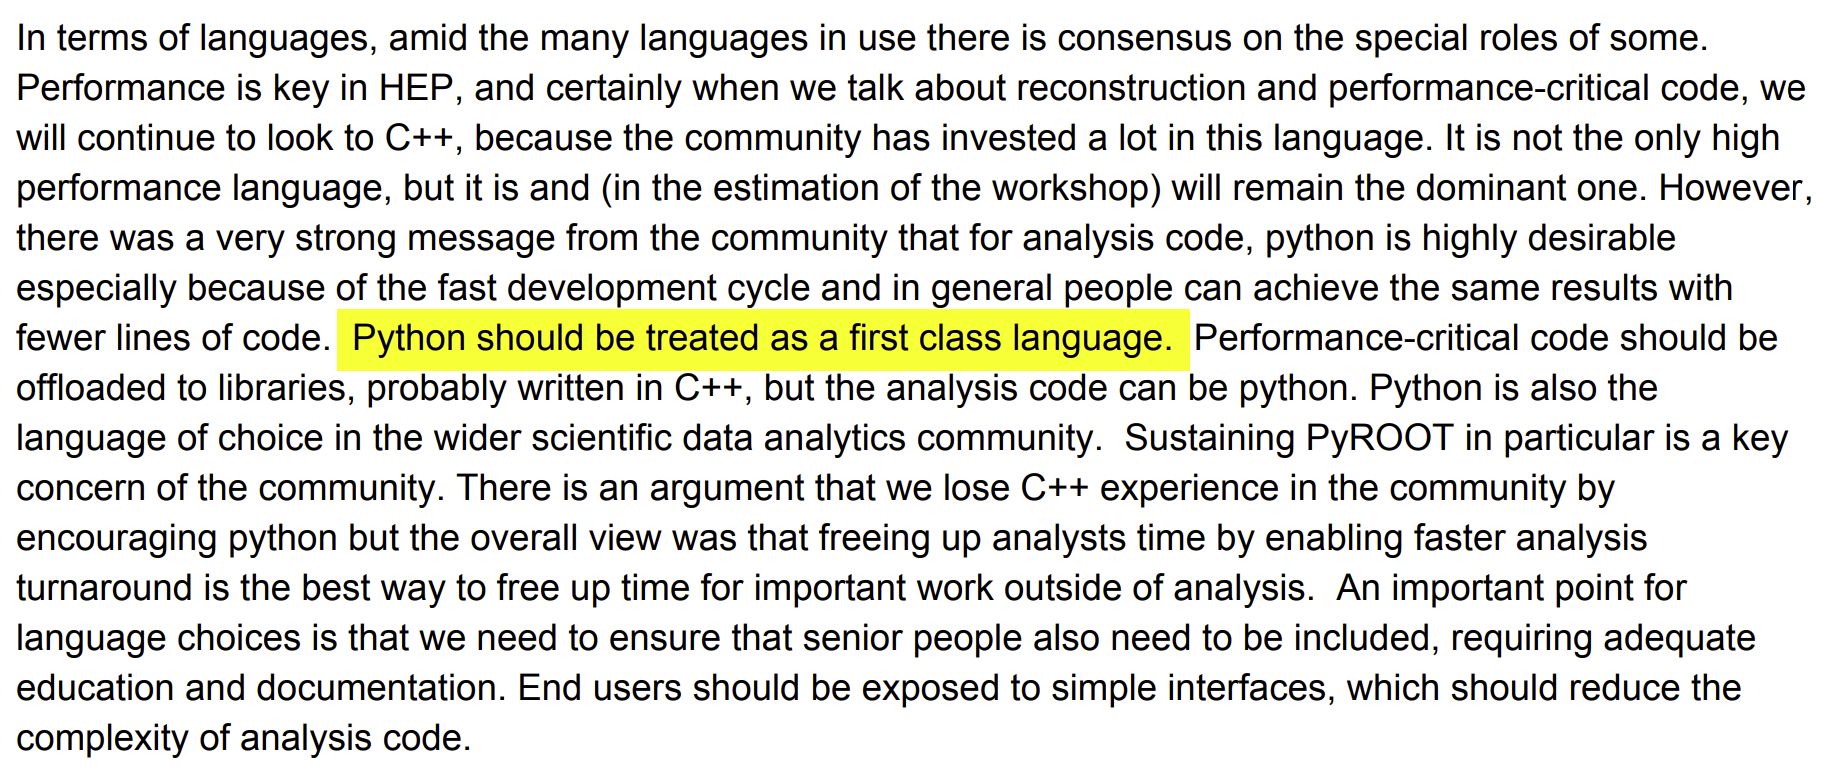
\includegraphics[width=\linewidth]{PLOTS/ecosystem-2017-python-first-class-2.png}
\end{columns}
\end{frame}

\begin{frame}{Back then, Python was just beginning to take over data analytics}
\vspace{0.25 cm}
\textcolor{darkblue}{Source: Google Analytics, worldwide search traffic.}

\vspace{-0.3 cm}
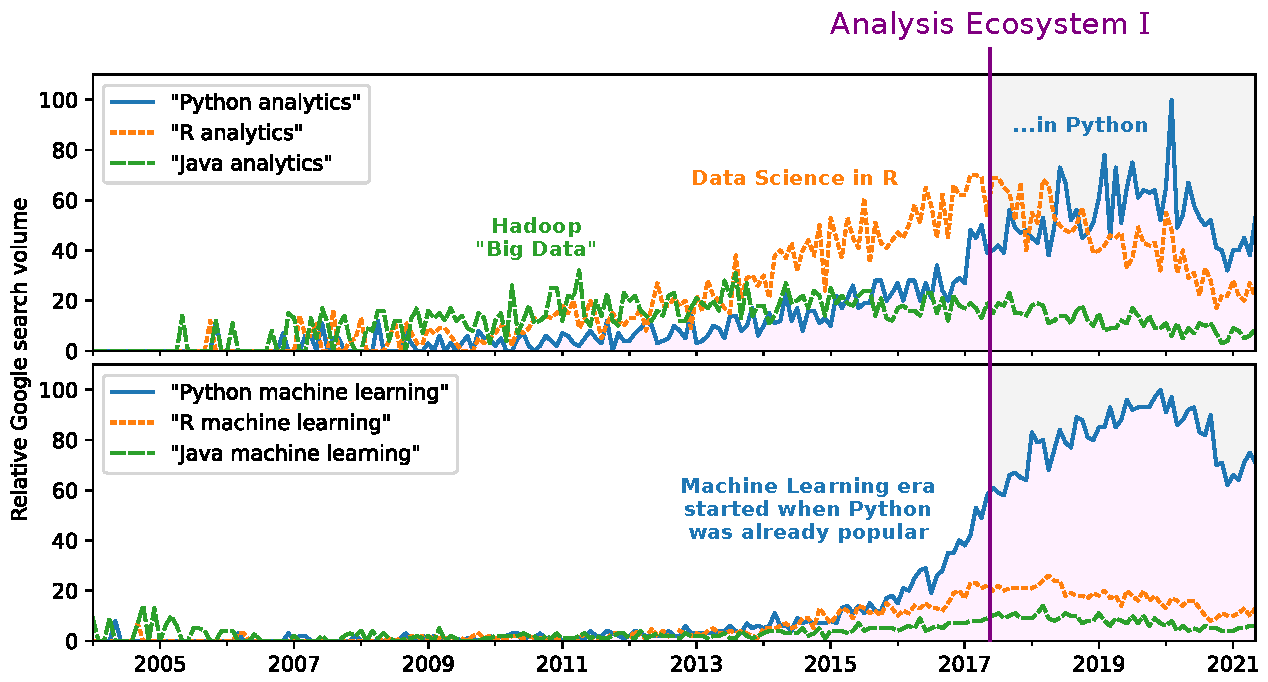
\includegraphics[width=\linewidth]{PLOTS/analytics-by-language.pdf}
\end{frame}

\begin{frame}{Though it had been slowly growing in HEP for years}
\vspace{0.25 cm}
\textcolor{darkblue}{Source: Title and abstract matches in CHEP proceedings.}

\vspace{-0.3 cm}
\mbox{ } \hfill 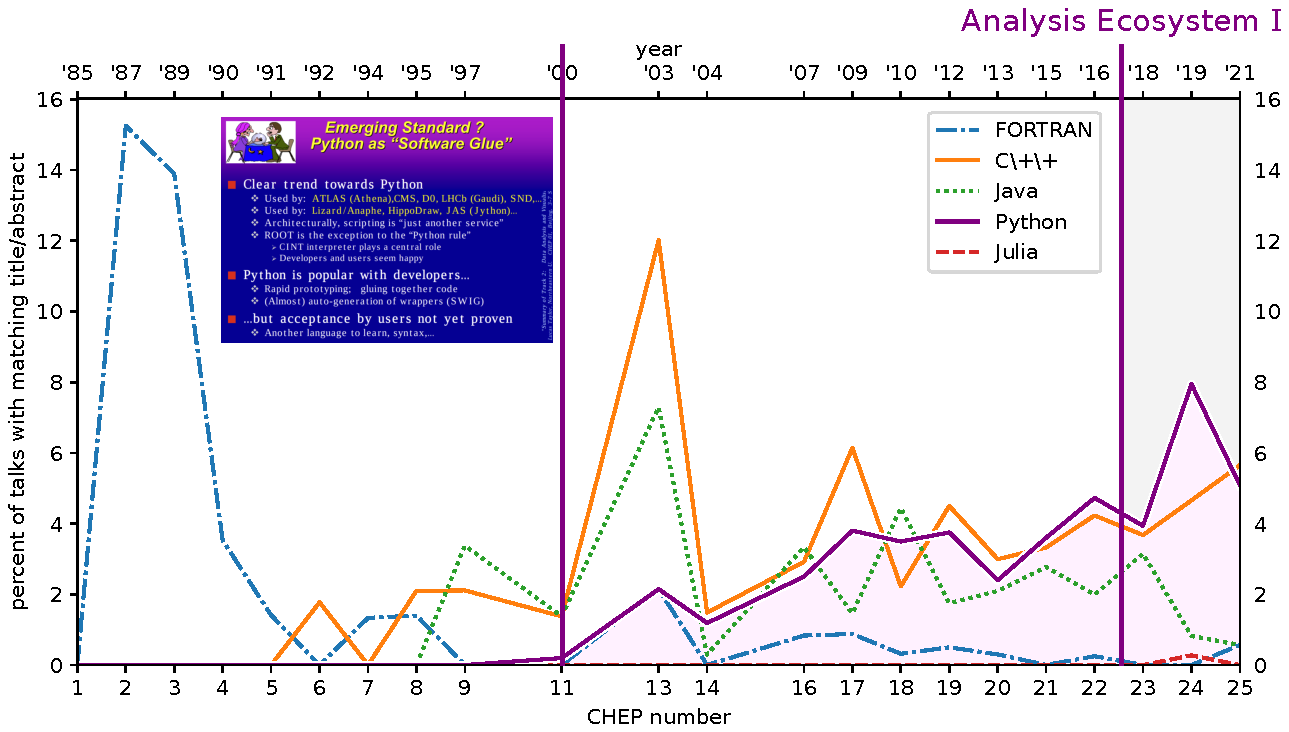
\includegraphics[width=0.95\linewidth]{PLOTS/chep-papers-language-2.pdf} \hfill \mbox{ }
\end{frame}

\begin{frame}{But the use of Scientific Python (NumPy, etc.) was new to HEP}
\vspace{0.25 cm}
\textcolor{darkblue}{Source: ``\mintinline{python}{import XYZ}'' matches in GitHub repos for users who fork CMSSW.}

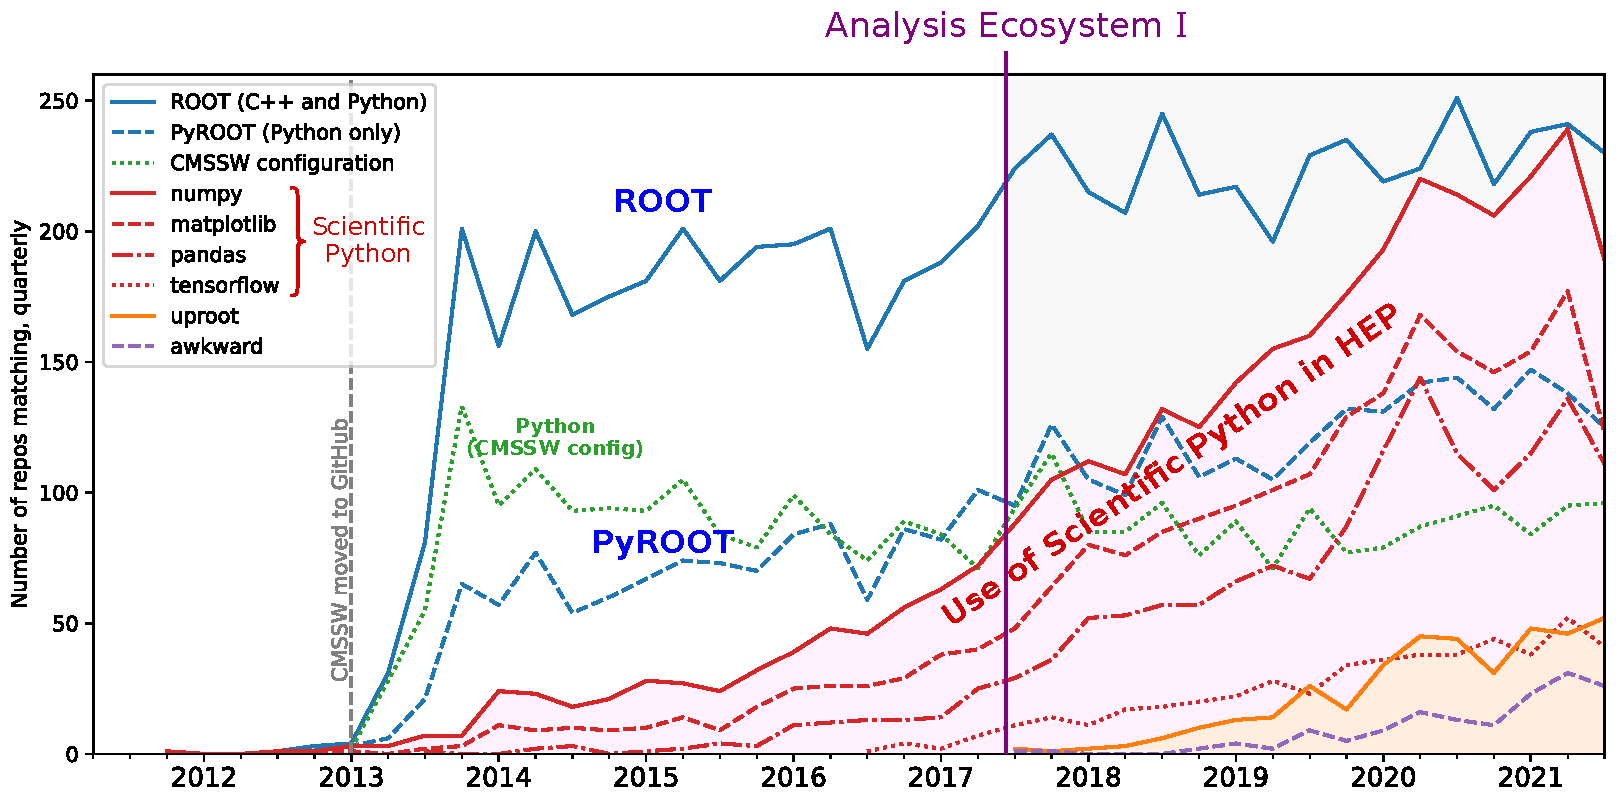
\includegraphics[width=\linewidth]{PLOTS/gihub-package-fullstudy-for-review.pdf}
\end{frame}

\begin{frame}{Scikit-HEP had not yet taken off}
\vspace{0.25 cm}
\textcolor{darkblue}{Source: ``\mintinline{bash}{pip install XYZ}'' download rate for MacOS/Windows (no batch jobs).}

\vspace{0.1 cm}
\only<1>{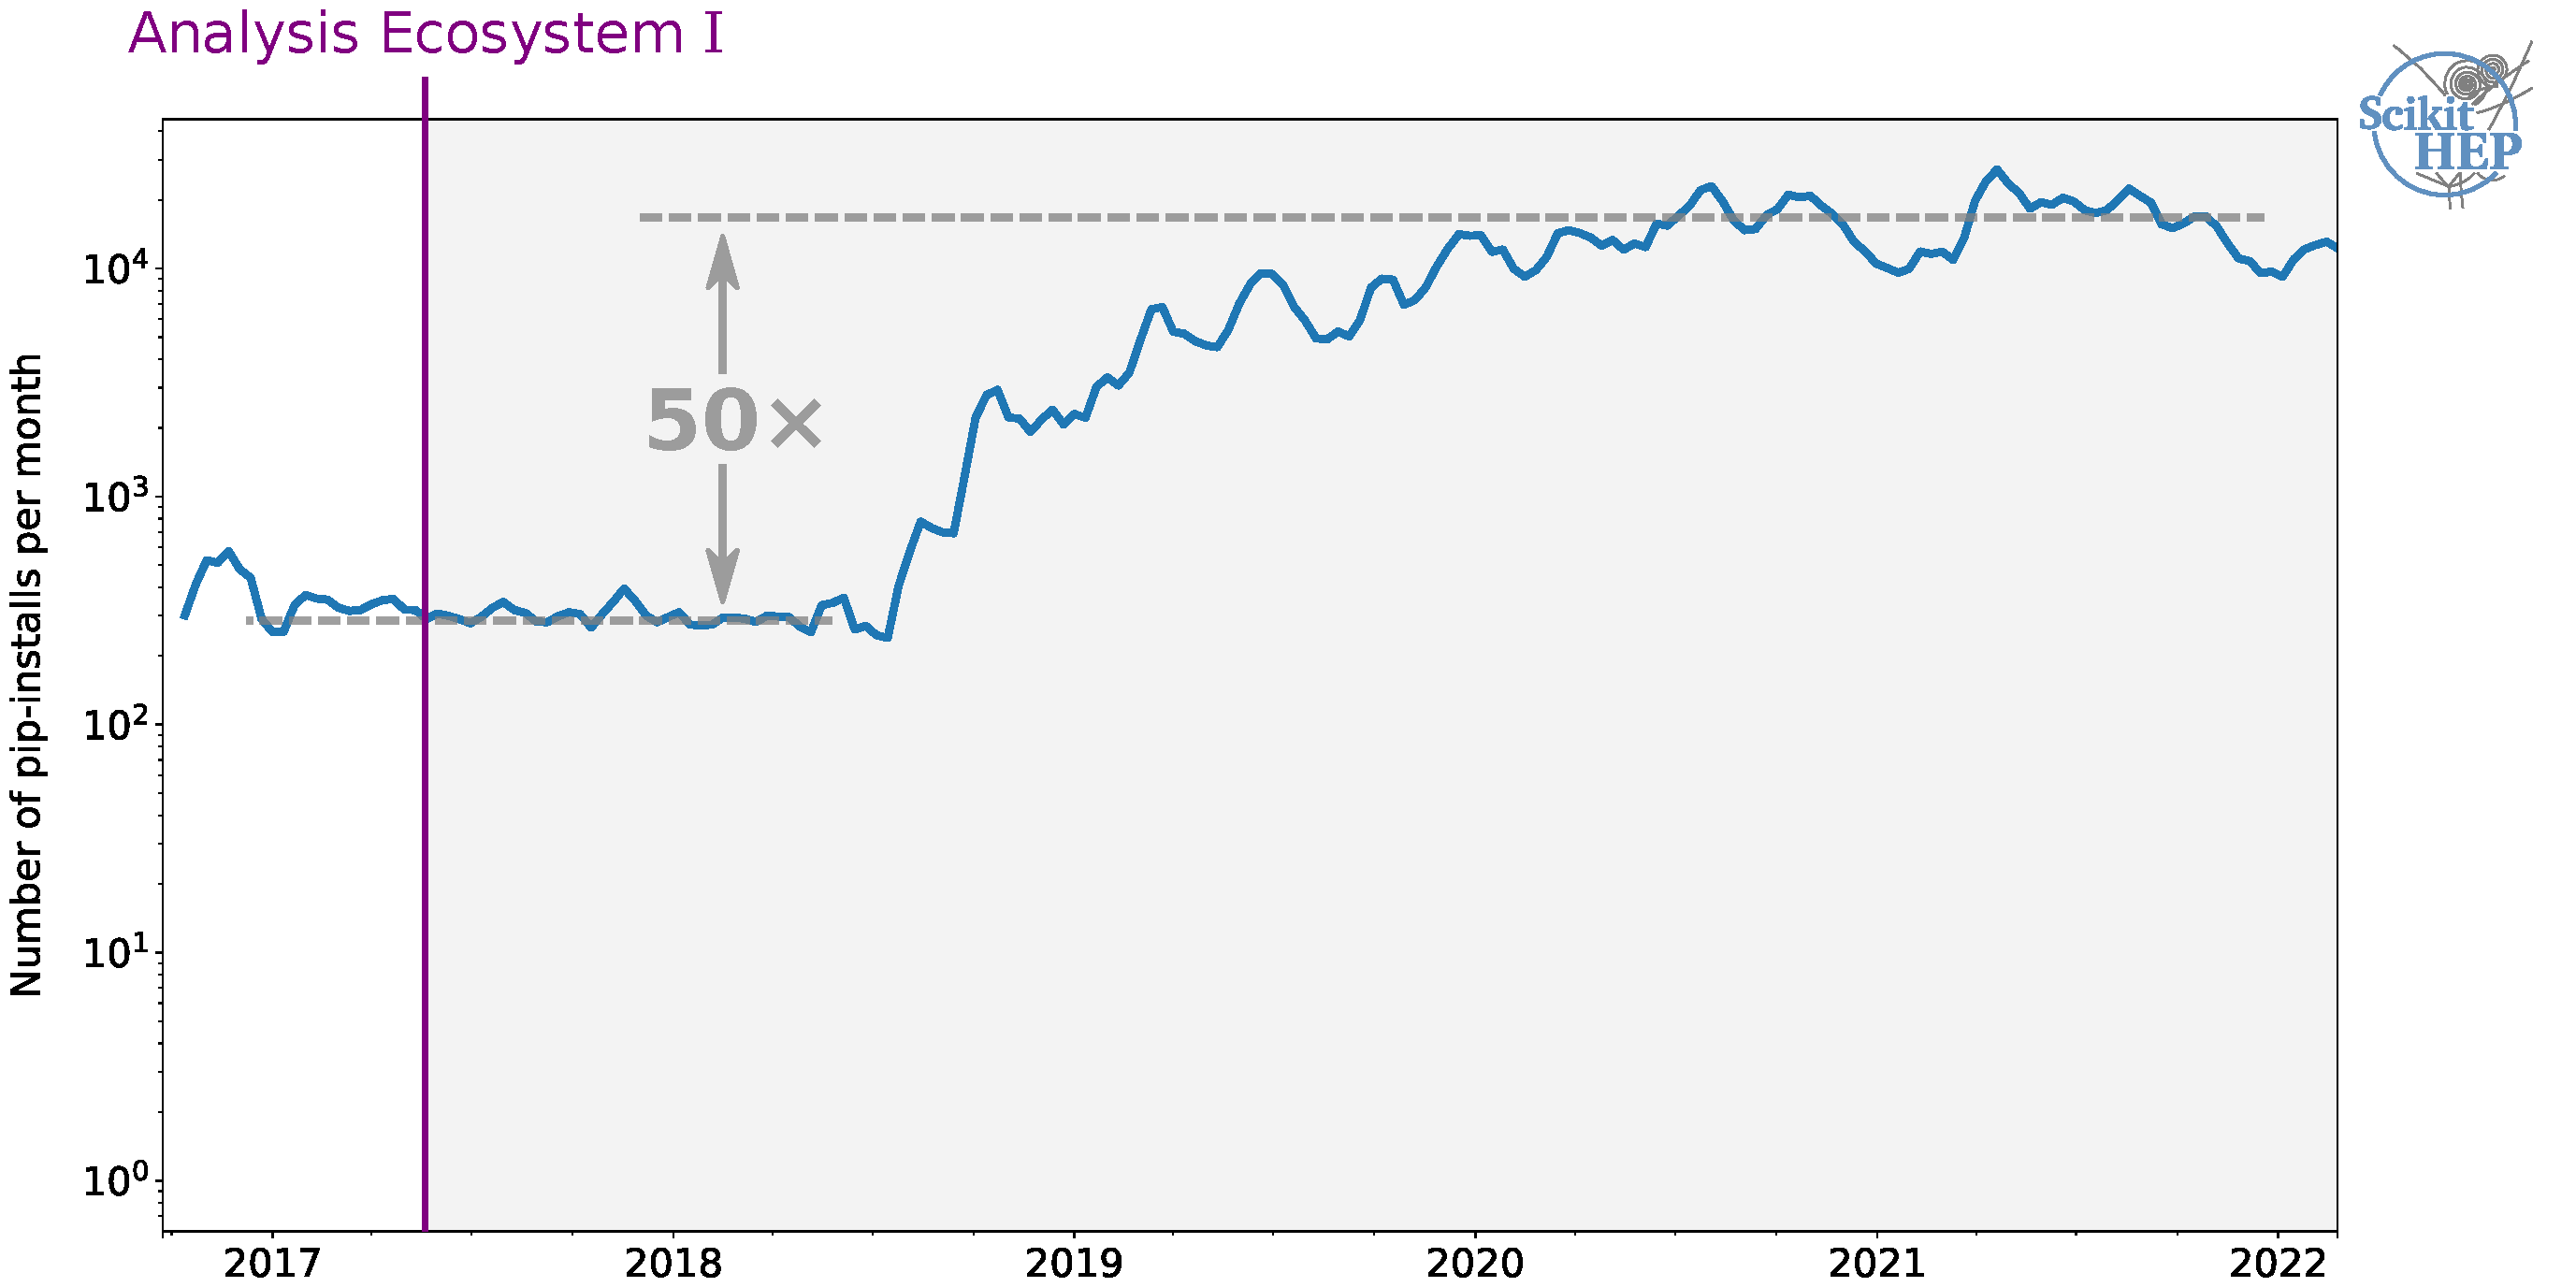
\includegraphics[width=\linewidth]{PLOTS/pip-macwin-scikithep-log-for-report-0.pdf}}\only<2>{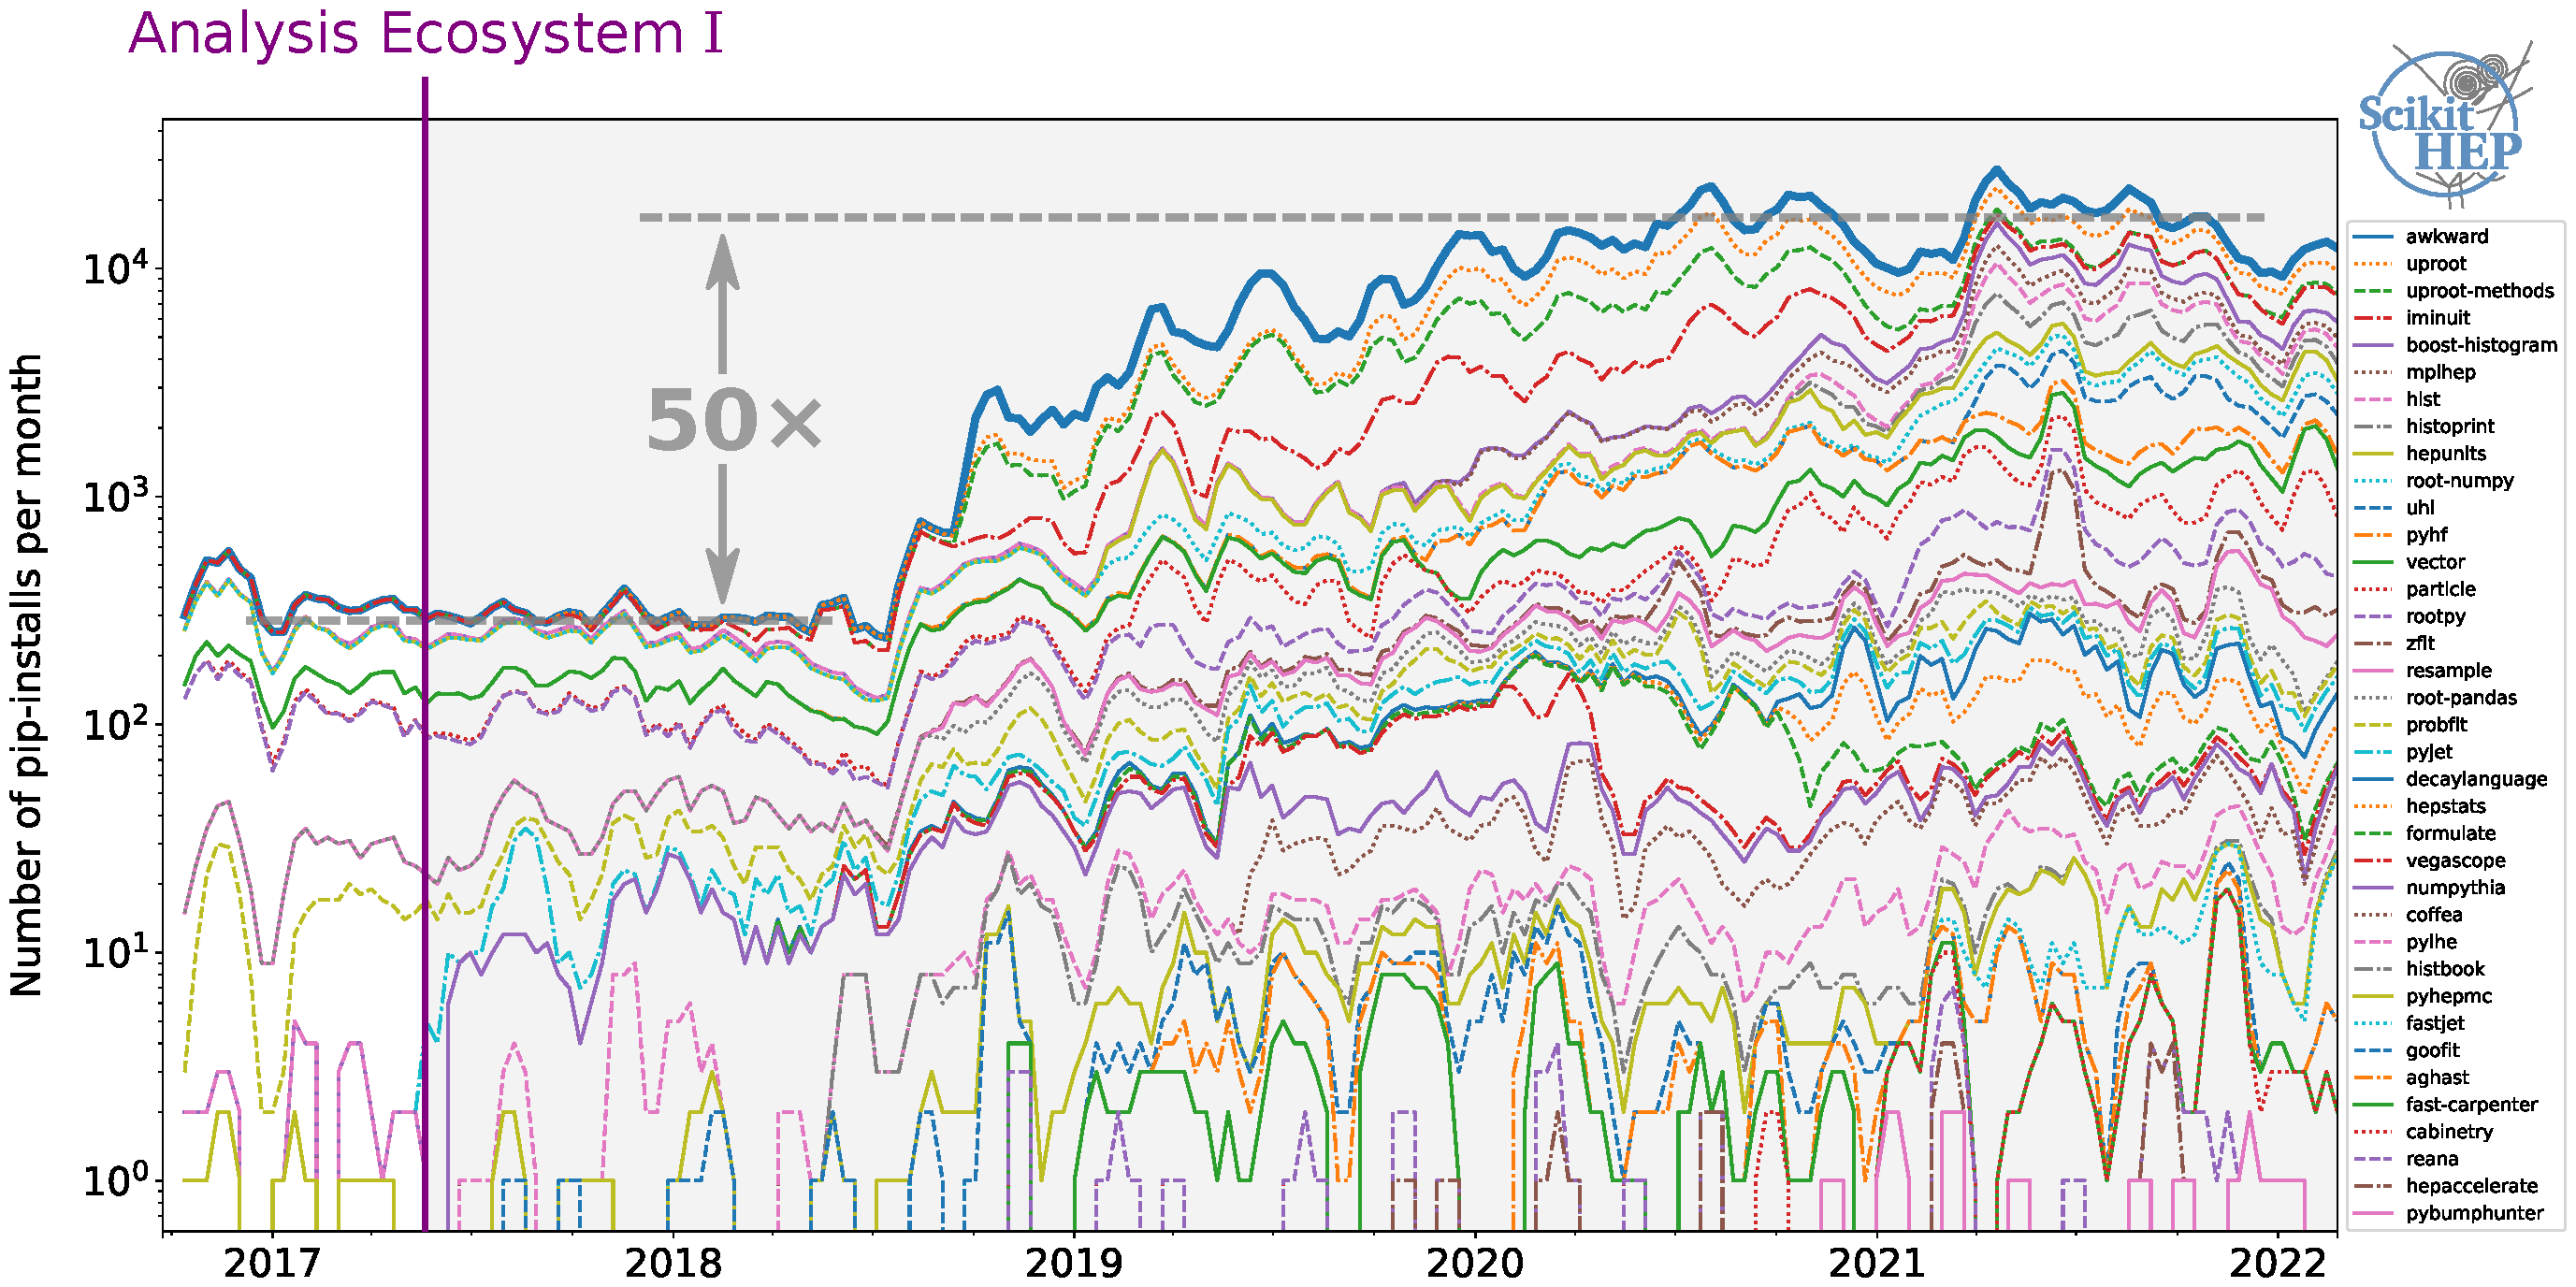
\includegraphics[width=\linewidth]{PLOTS/pip-macwin-scikithep-log-for-report.pdf}}
\end{frame}

\begin{frame}{We are now a two-language community}
\vspace{0.25 cm}
\textcolor{darkblue}{Source: PyHEP 2020 workshop survey.}

\vspace{-0.3 cm}
\begin{columns}
\column{1.15\linewidth}
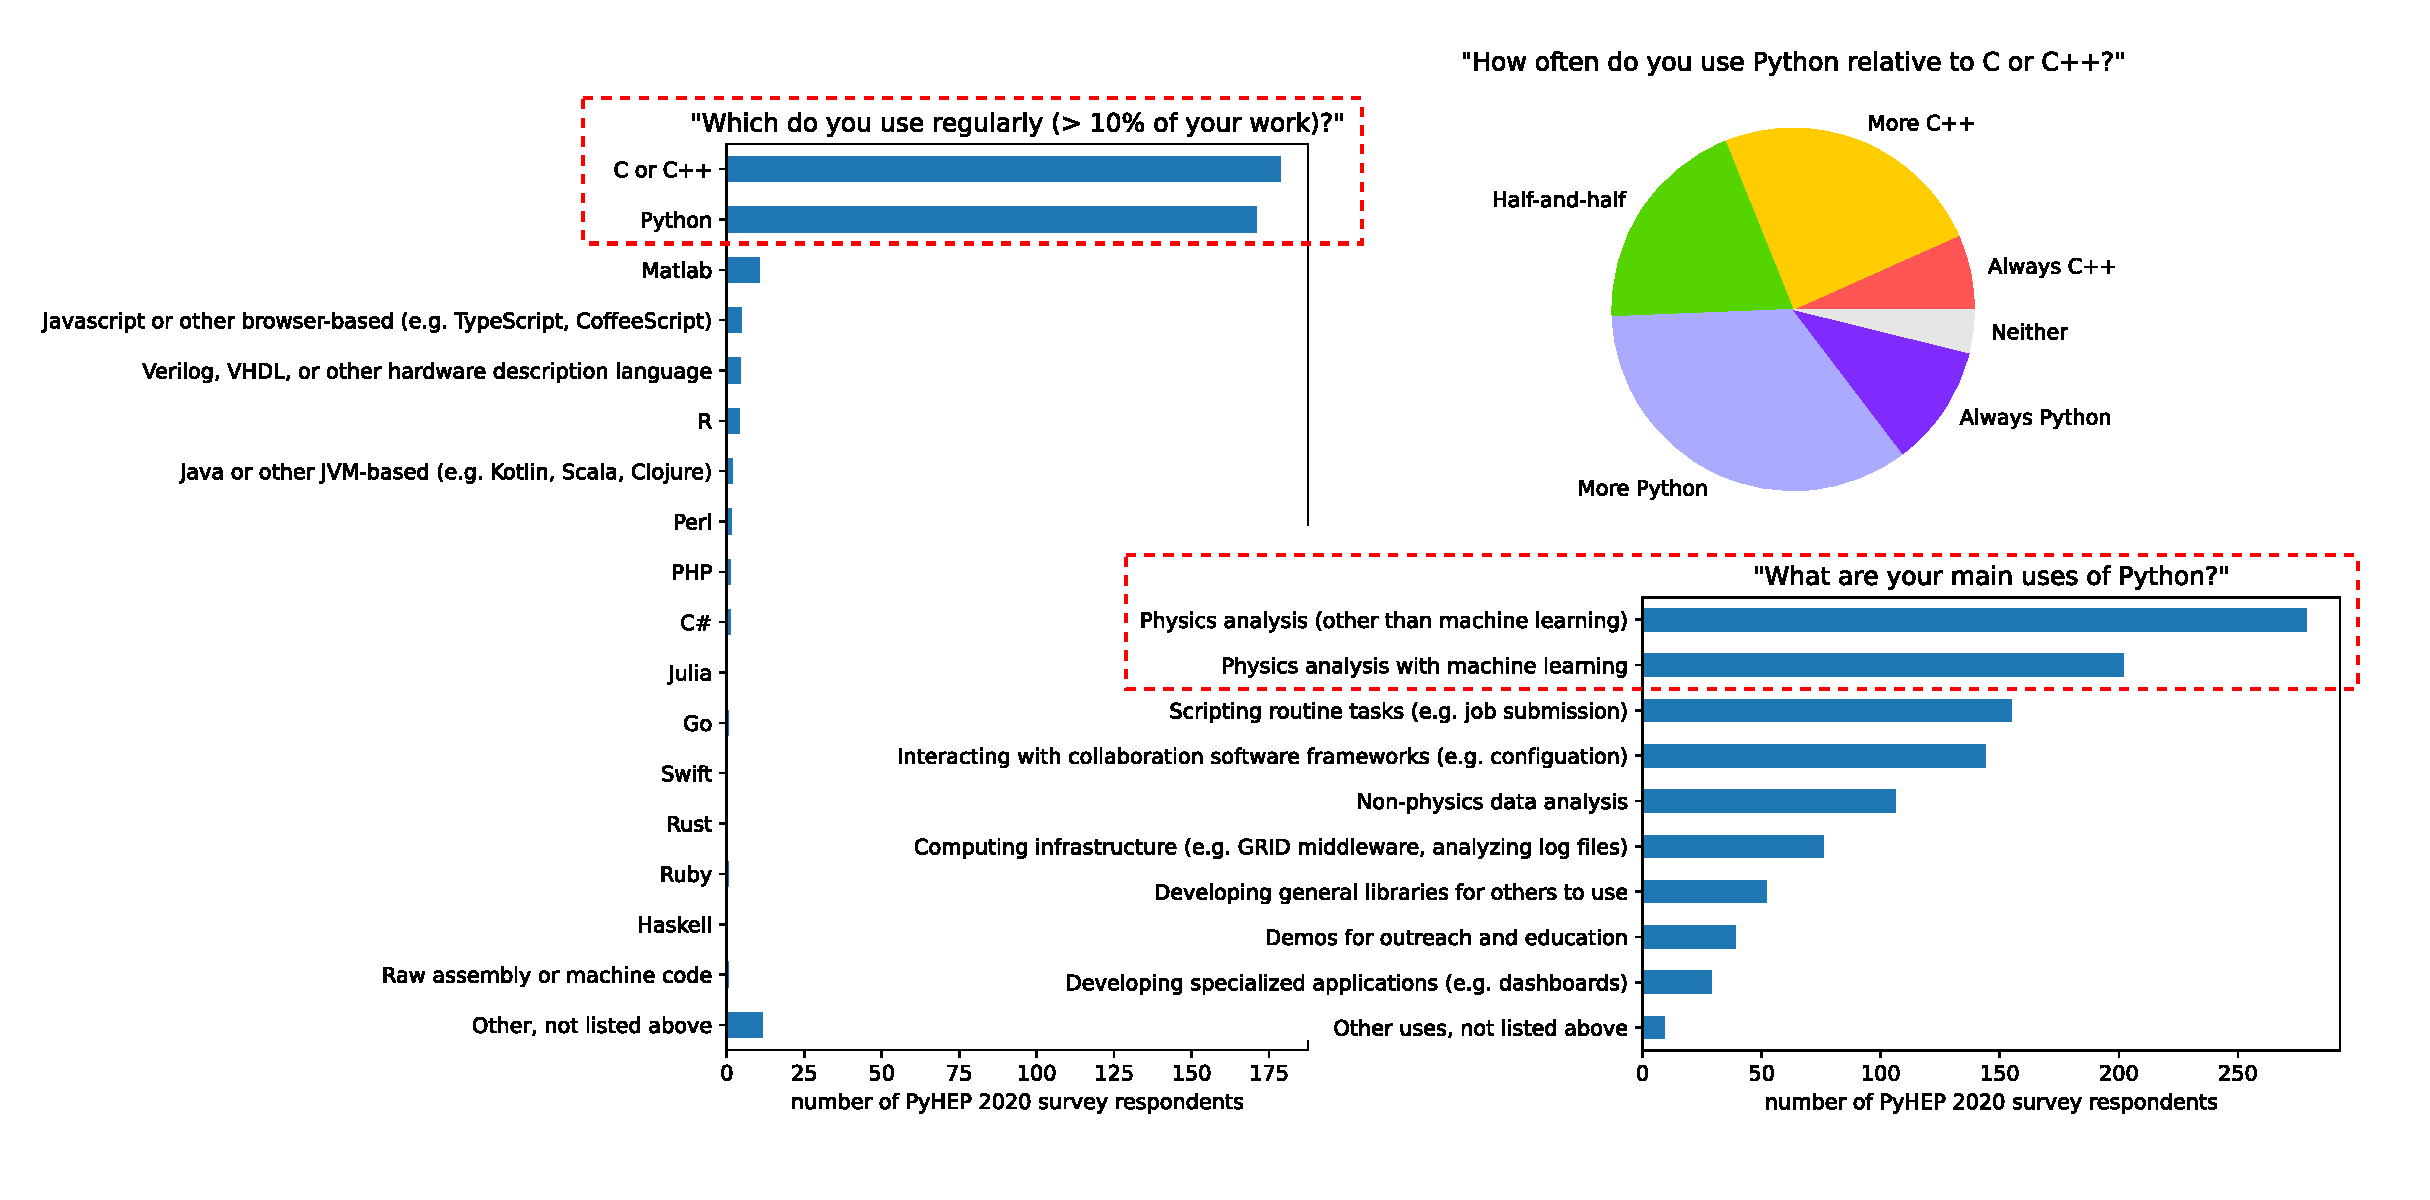
\includegraphics[width=\linewidth]{PLOTS/pyhep2020-survey-5.pdf}
\end{columns}
\end{frame}

\begin{frame}{The Pythonic HEP ecosystem now}
\begin{center}
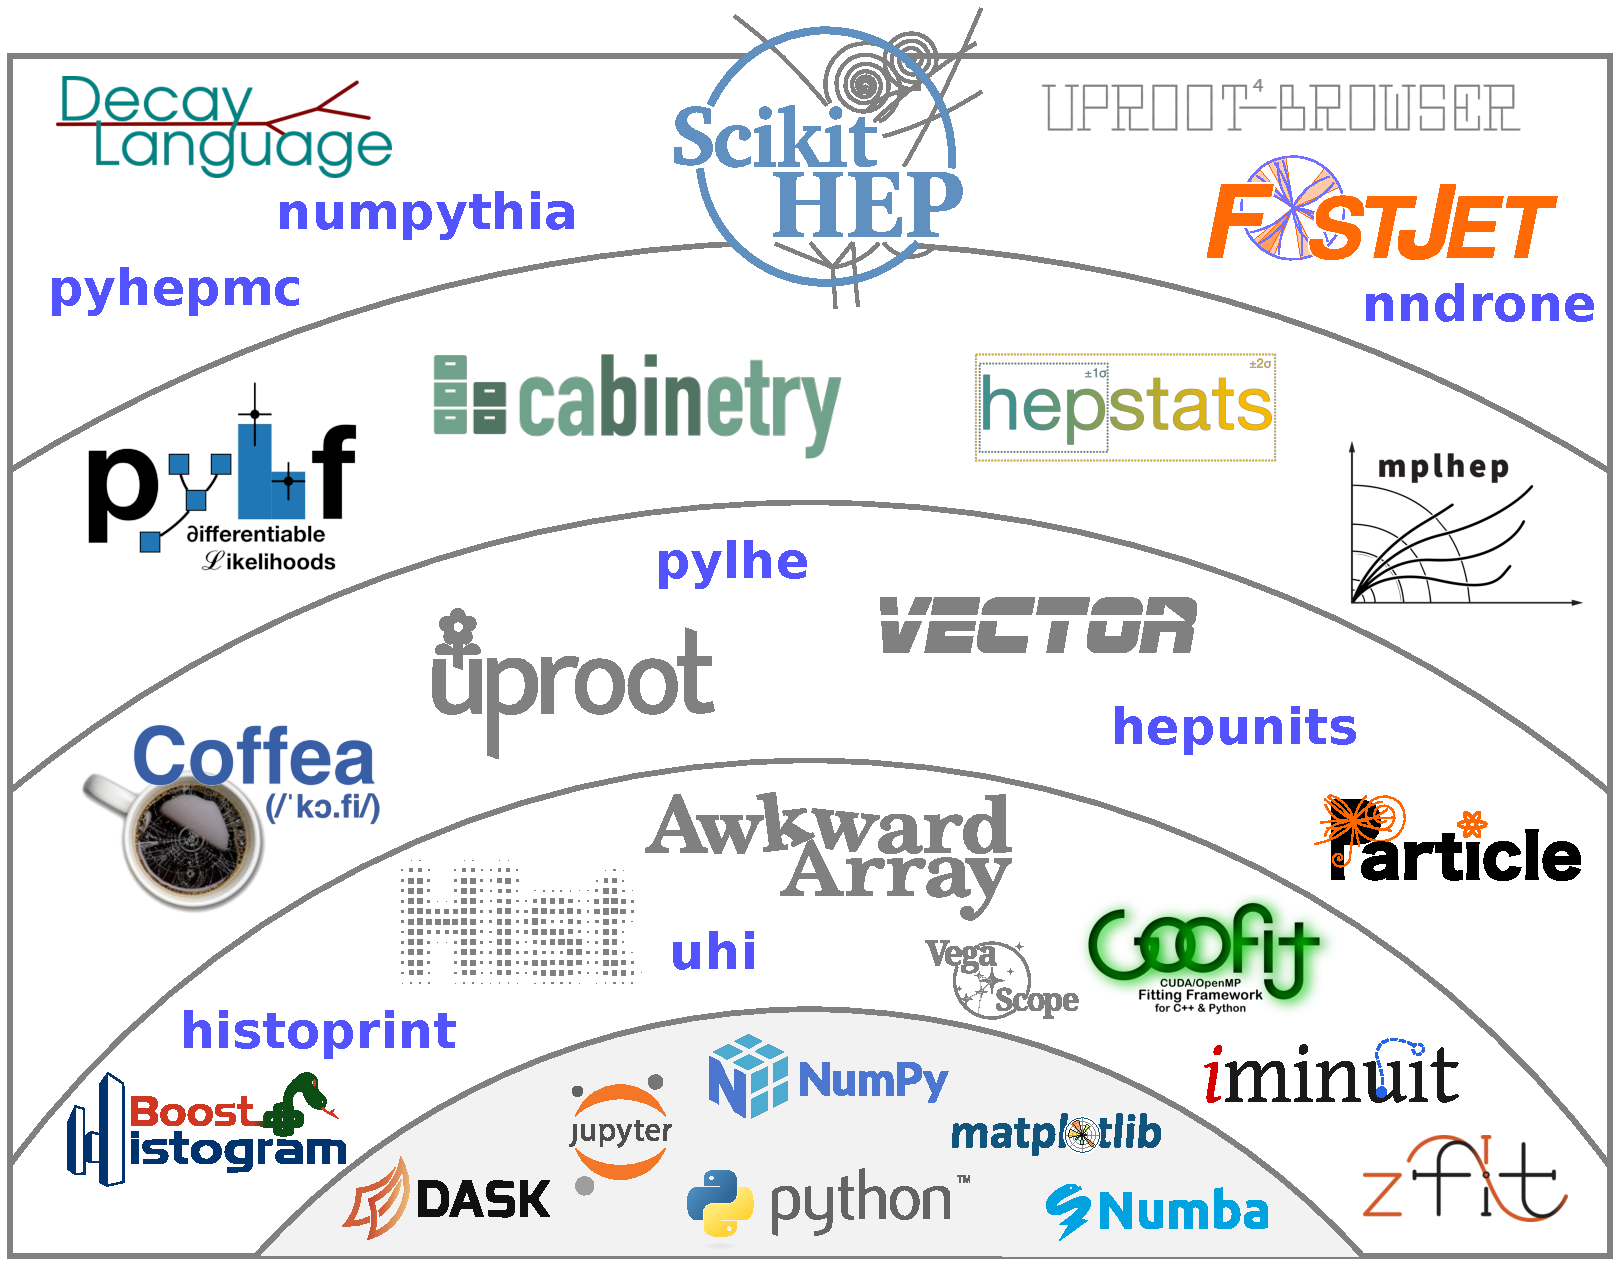
\includegraphics[width=0.72\linewidth]{PLOTS/shells-hep.pdf}
\end{center}
\end{frame}

\begin{frame}{Case study: convergence of histogram libraries}
\vspace{0.5 cm}
The Scientific Python world lacked HEP-style histograms; it's one of the things we have to make ourselves.

\vspace{0.5 cm}
\uncover<2->{Also, it seems easy: just bin and count, right?}

\vspace{0.5 cm}
\uncover<3->{Physicists have created at least 20 histogram libraries in Python, most single-author.}

\vspace{0.5 cm}
\begin{uncoverenv}<3->
\begin{columns}
\scriptsize
\column{0.26\linewidth}
\begin{itemize}
\item PyROOT (2004--now)
\item PAIDA (2004--2007)
\item Plothon (2007--2008)
\item SVGFig (2008--2009)
\item YODA (2008--now)
\end{itemize}

\column{0.27\linewidth}
\begin{itemize}
\item DANSE (2009--2011)
\item rootpy (2011--2019)
\item SimpleHist (2011--2015)
\item pyhistogram (2015)
\item multihist (2015--now)
\end{itemize}

\column{0.28\linewidth}
\begin{itemize}
\item matplotlib-hep (2016)
\item QHist (2017--2019)
\item Physt (2016--now)
\item \mbox{Histogrammar (2016--now)\hspace{-0.2 cm}}
\item HistBook (2018--2019)
\end{itemize}

\column{0.32\linewidth}
\begin{itemize}
\item Coffea.hist (2019--2022)
\item boost-histogram (2019--now)
\item mplhep (2019--now)
\item histoprint (2020--now)
\item hist (2020--now)
\end{itemize}

\end{columns}
\end{uncoverenv}
\end{frame}

\begin{frame}{Histogram proliferation and convergence}
\vspace{0.25 cm}
\textcolor{darkblue}{Number of unique developers contributing to each library per month (in git).}

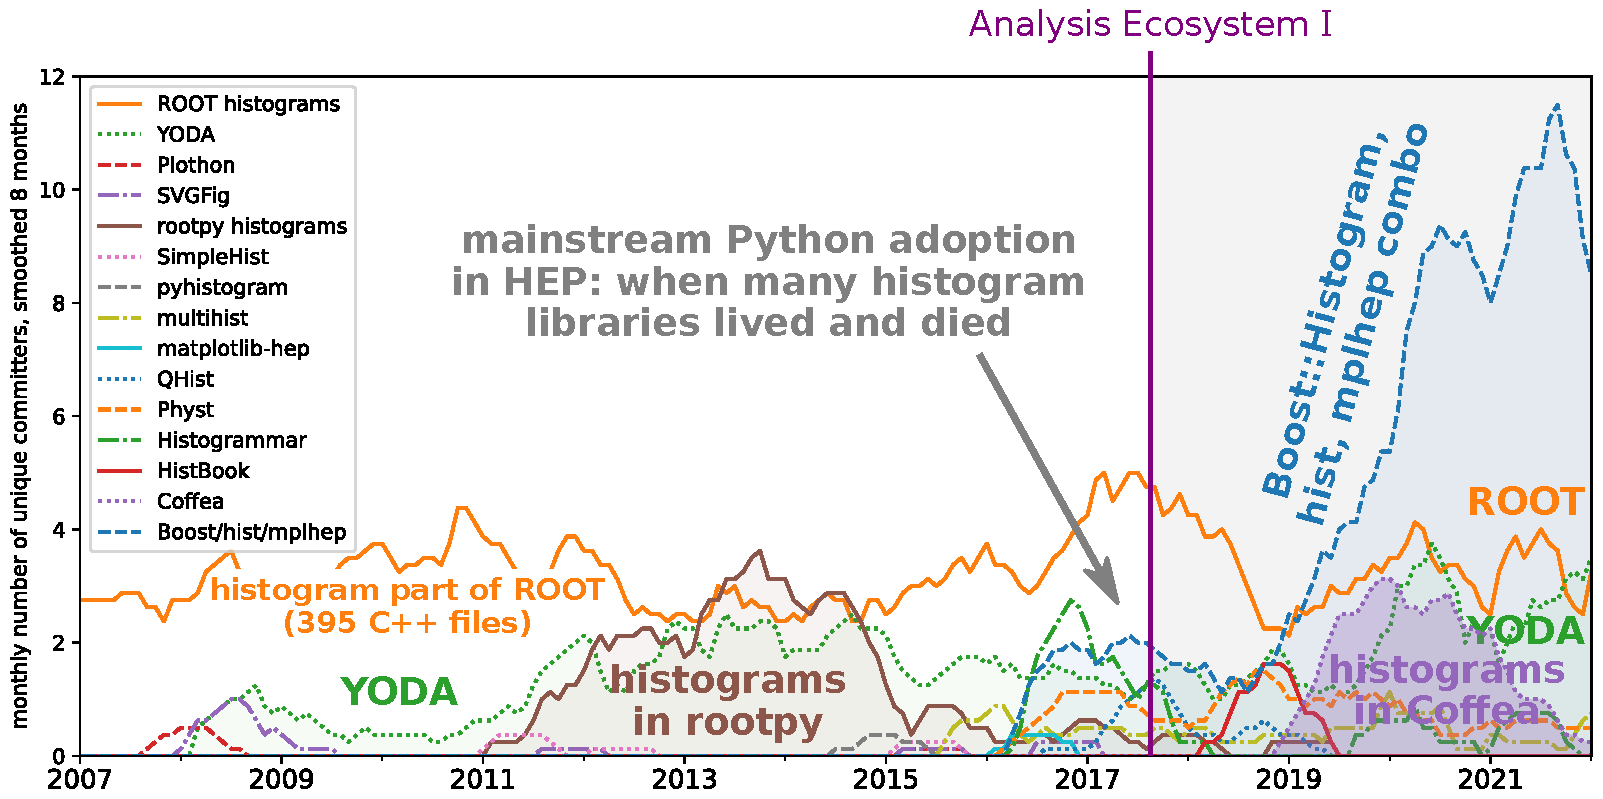
\includegraphics[width=\linewidth]{PLOTS/github-histogram-libraries.pdf}
\end{frame}

\begin{frame}[fragile]{Why combine Boost::Histogram, hist, mplhep?}
\vspace{0.5 cm}
\begin{columns}
\column{0.6\linewidth}
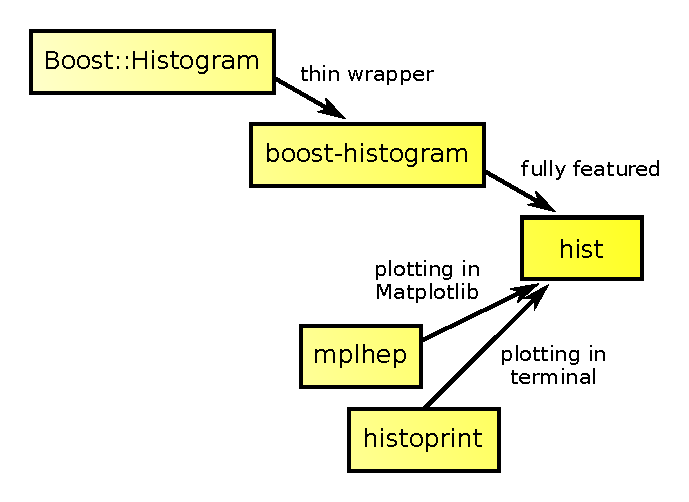
\includegraphics[width=\linewidth]{PLOTS/histogram-convergence.pdf}

\column{0.45\linewidth}
Originally, each of these was developed independently by a single author.

\vspace{0.75 cm}
\begin{uncoverenv}<2->
They each provide a piece of functionality users can get through

\begin{minted}{python}
import hist
\end{minted}
\end{uncoverenv}

\vspace{0.75 cm}
\uncover<3->{Now, 47 developers have contributed to these packages, and 20 contributed to more than one.}
\end{columns}
\end{frame}

\begin{frame}{Consistency maintained through agreed-upon protocols}
\vspace{0.5 cm}
\begin{columns}
\column{1.1\linewidth}
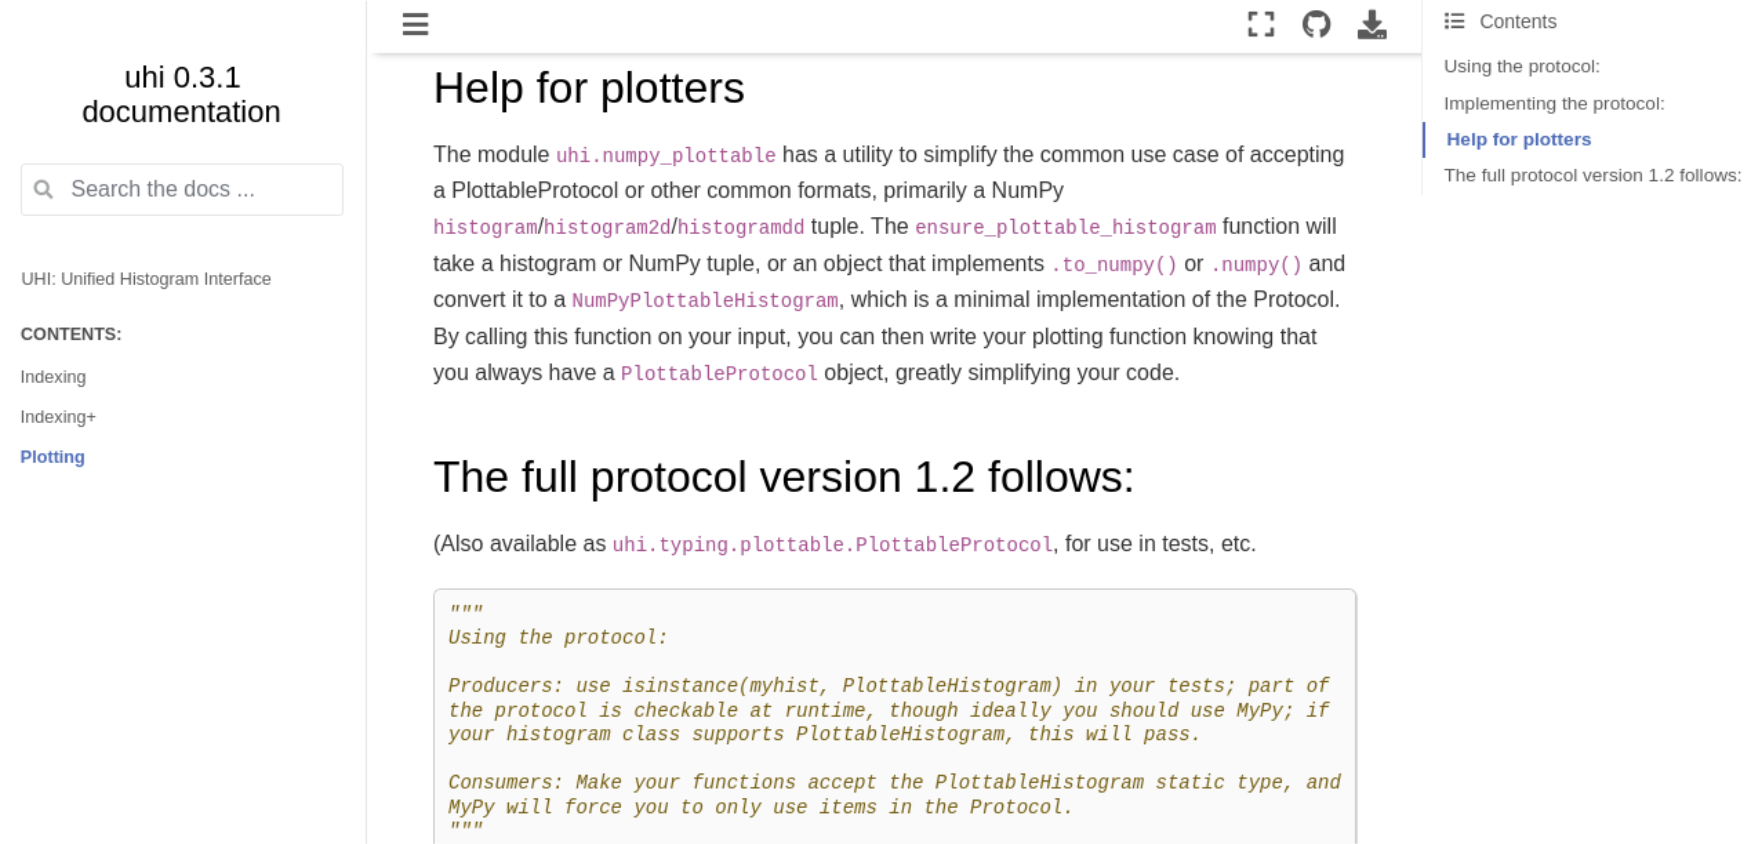
\includegraphics[width=\linewidth]{PLOTS/histogram-protocol-screenshot.png}
\end{columns}
\end{frame}

\begin{frame}{uproot-browser: another interface package that pulls many together}
\vspace{0.35 cm}
\begin{center}
\only<1>{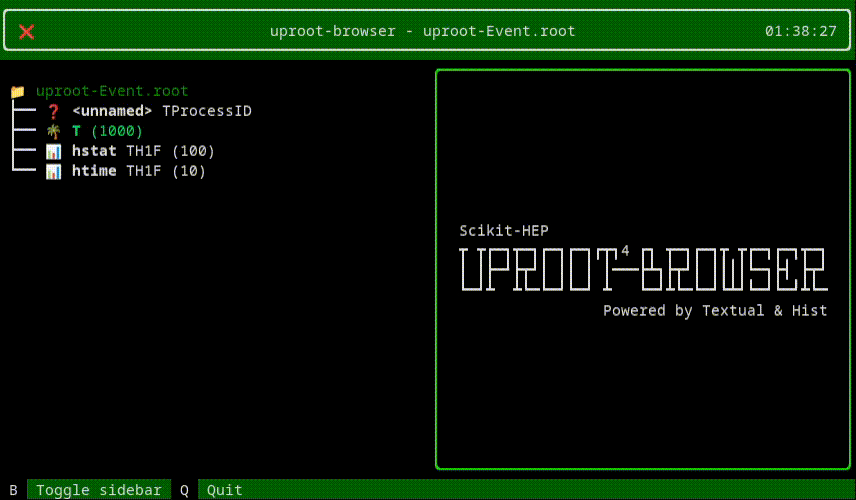
\includegraphics[width=0.9\linewidth]{PLOTS/uproot-browser-tui-frames/00.png}}\only<2>{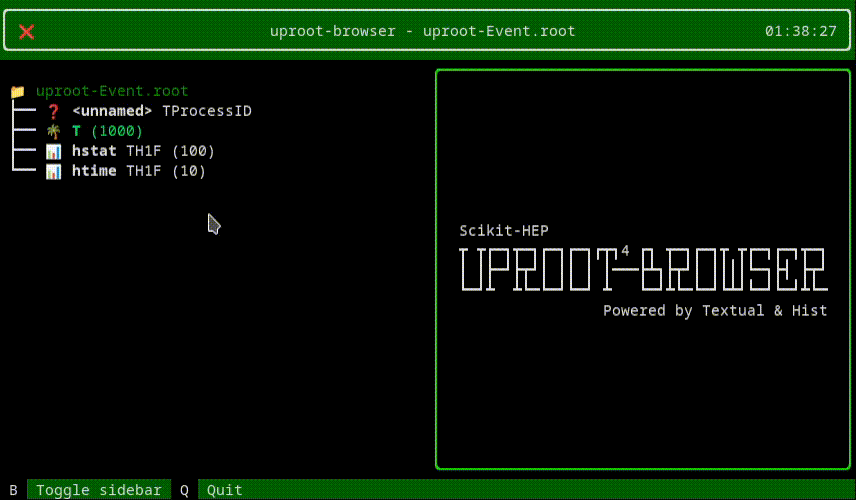
\includegraphics[width=0.9\linewidth]{PLOTS/uproot-browser-tui-frames/01.png}}\only<3>{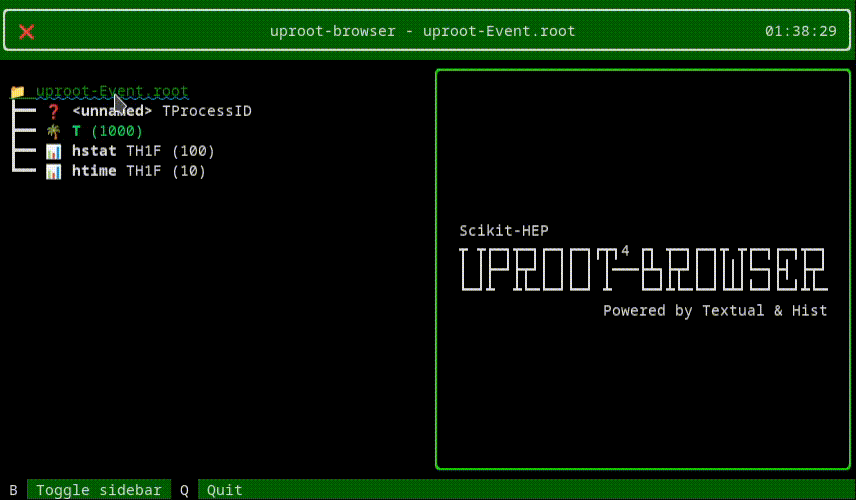
\includegraphics[width=0.9\linewidth]{PLOTS/uproot-browser-tui-frames/02.png}}\only<4>{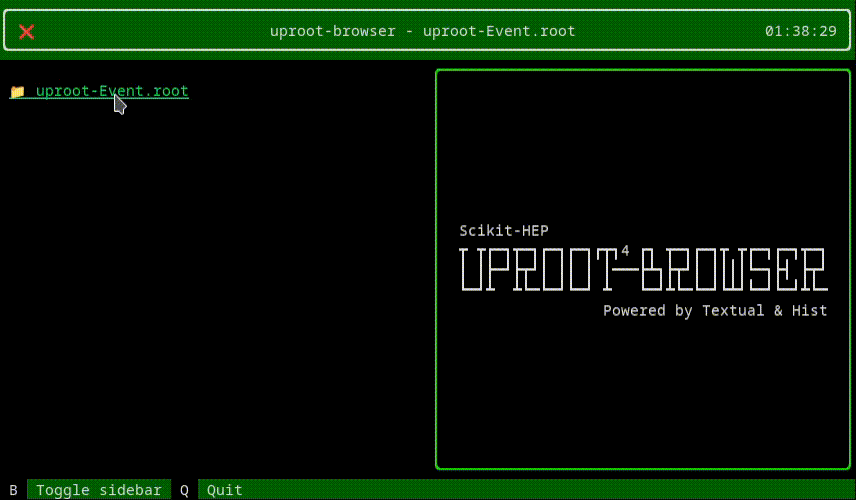
\includegraphics[width=0.9\linewidth]{PLOTS/uproot-browser-tui-frames/03.png}}\only<5>{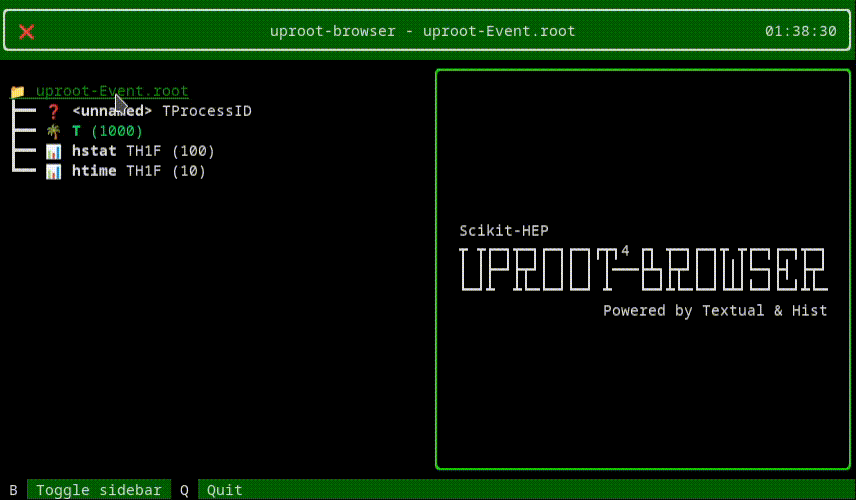
\includegraphics[width=0.9\linewidth]{PLOTS/uproot-browser-tui-frames/04.png}}\only<6>{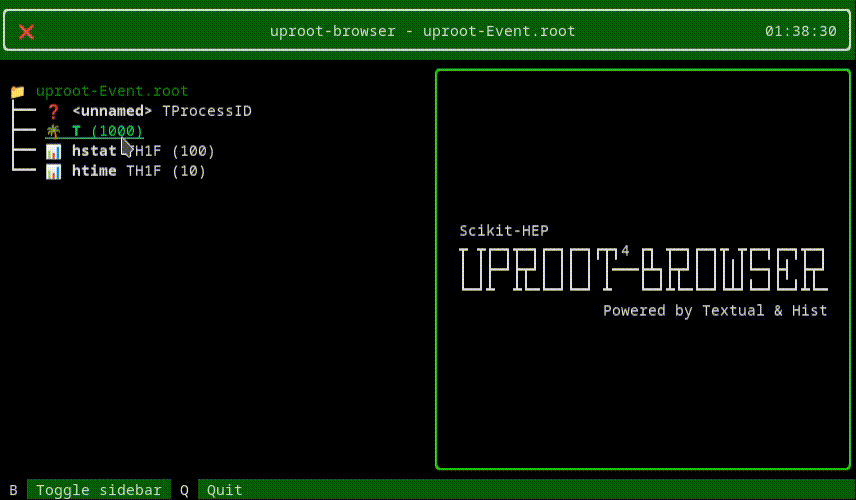
\includegraphics[width=0.9\linewidth]{PLOTS/uproot-browser-tui-frames/05.png}}\only<7>{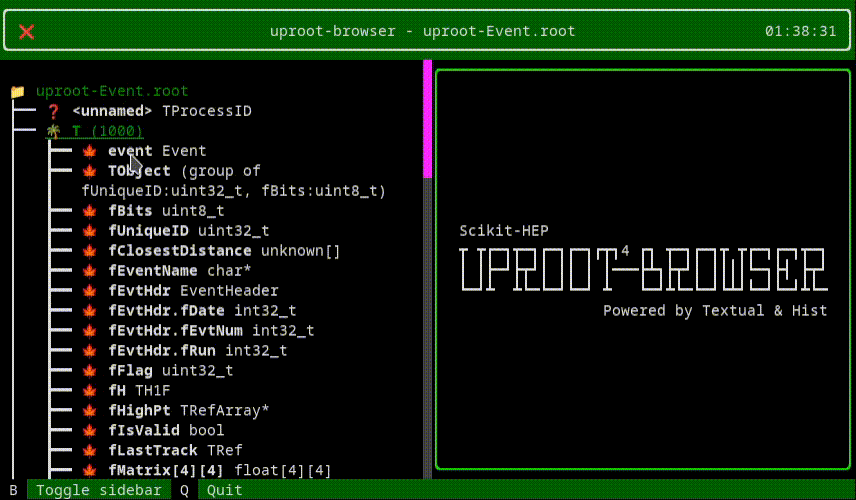
\includegraphics[width=0.9\linewidth]{PLOTS/uproot-browser-tui-frames/06.png}}\only<8>{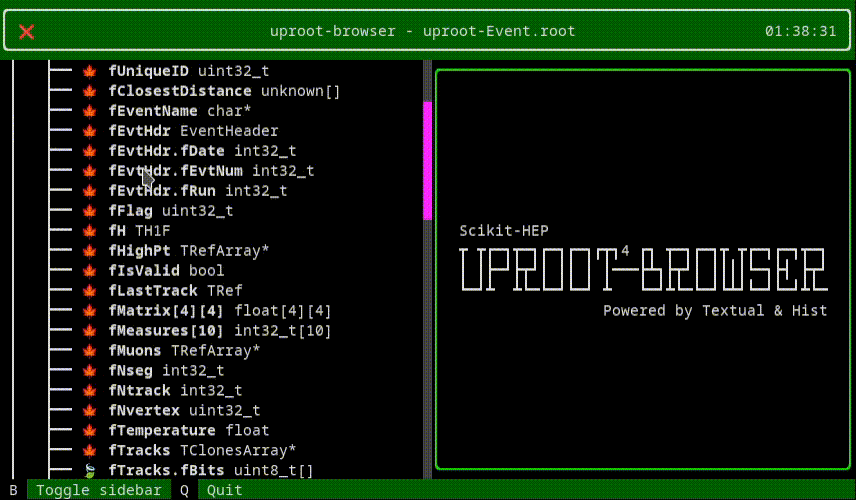
\includegraphics[width=0.9\linewidth]{PLOTS/uproot-browser-tui-frames/07.png}}\only<9>{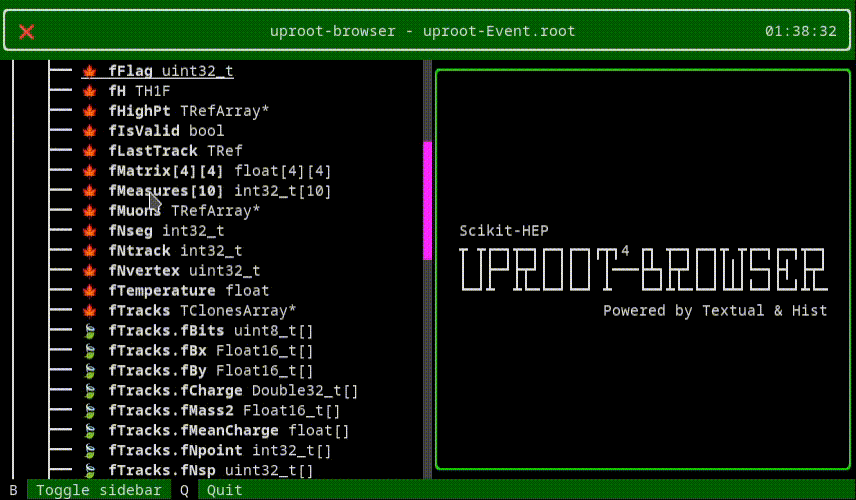
\includegraphics[width=0.9\linewidth]{PLOTS/uproot-browser-tui-frames/08.png}}\only<10>{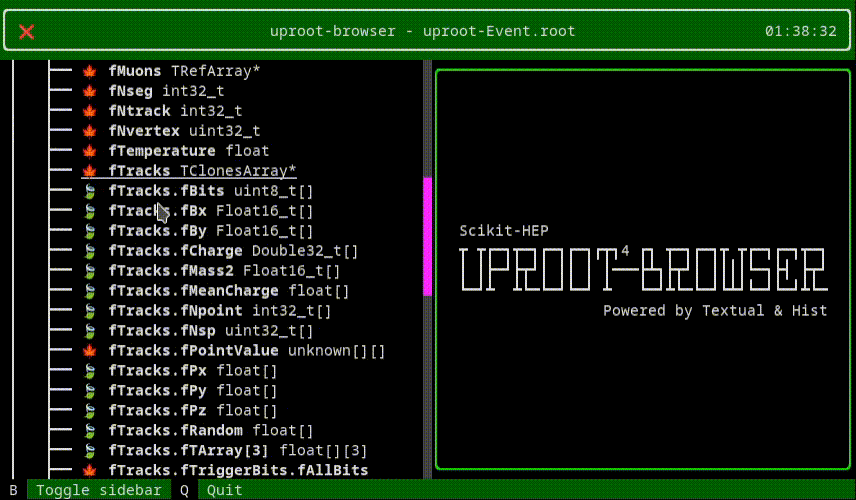
\includegraphics[width=0.9\linewidth]{PLOTS/uproot-browser-tui-frames/09.png}}\only<11>{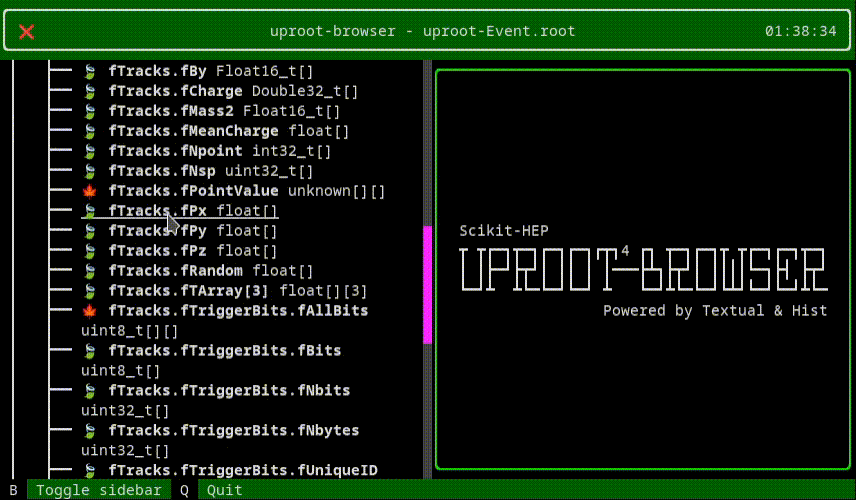
\includegraphics[width=0.9\linewidth]{PLOTS/uproot-browser-tui-frames/10.png}}\only<12>{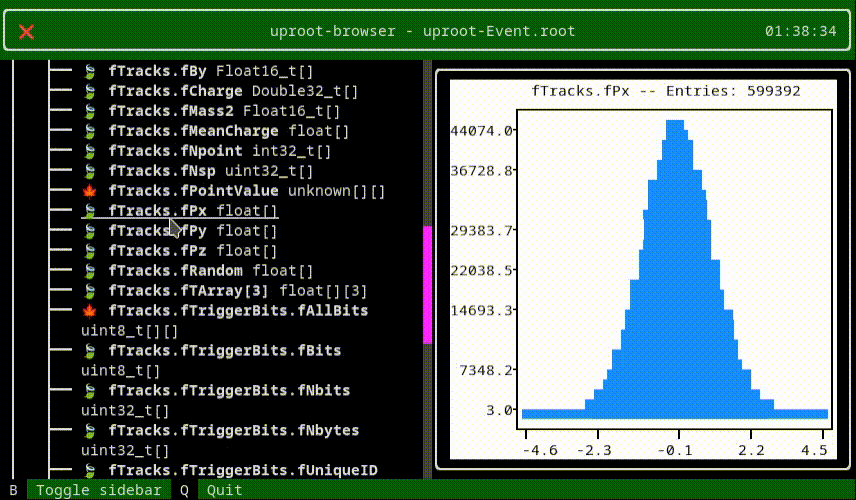
\includegraphics[width=0.9\linewidth]{PLOTS/uproot-browser-tui-frames/11.png}}\only<13>{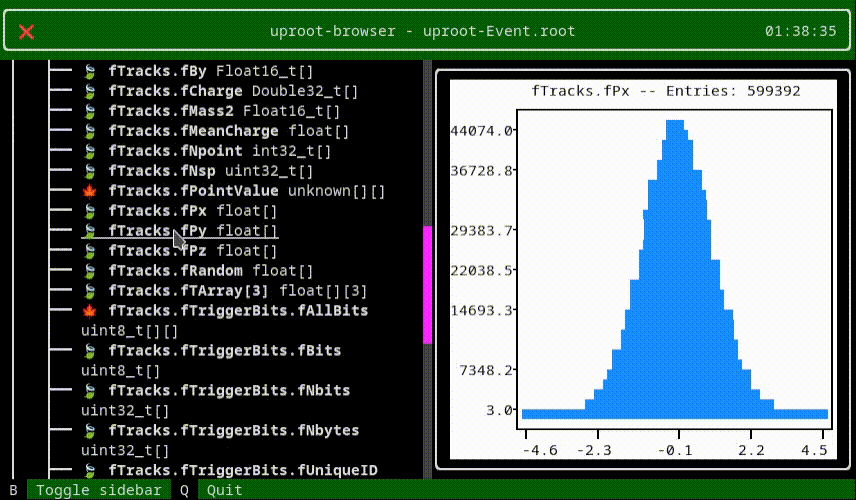
\includegraphics[width=0.9\linewidth]{PLOTS/uproot-browser-tui-frames/12.png}}\only<14>{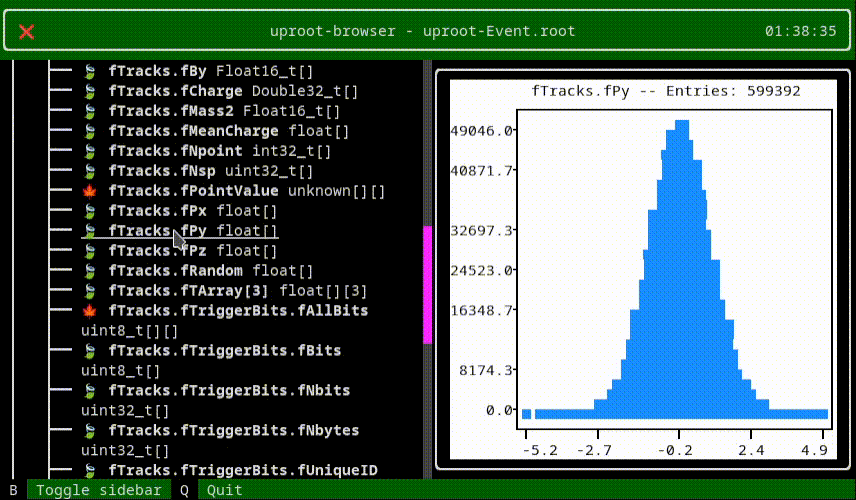
\includegraphics[width=0.9\linewidth]{PLOTS/uproot-browser-tui-frames/13.png}}\only<15>{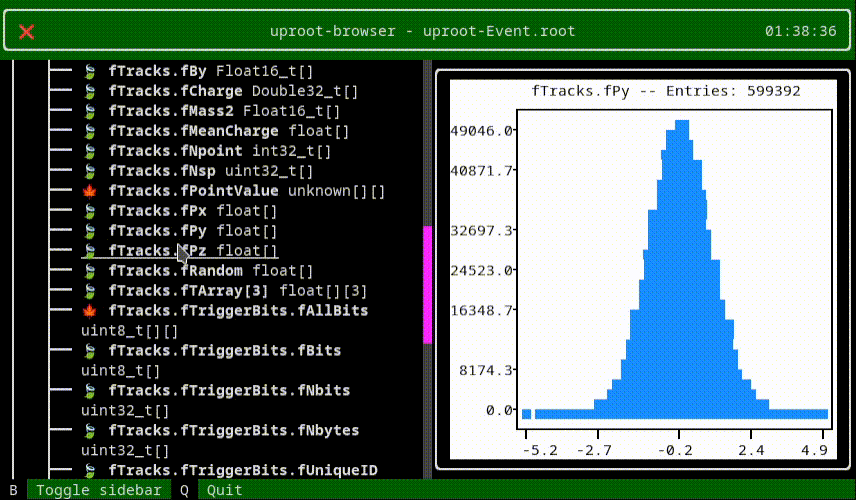
\includegraphics[width=0.9\linewidth]{PLOTS/uproot-browser-tui-frames/14.png}}\only<16>{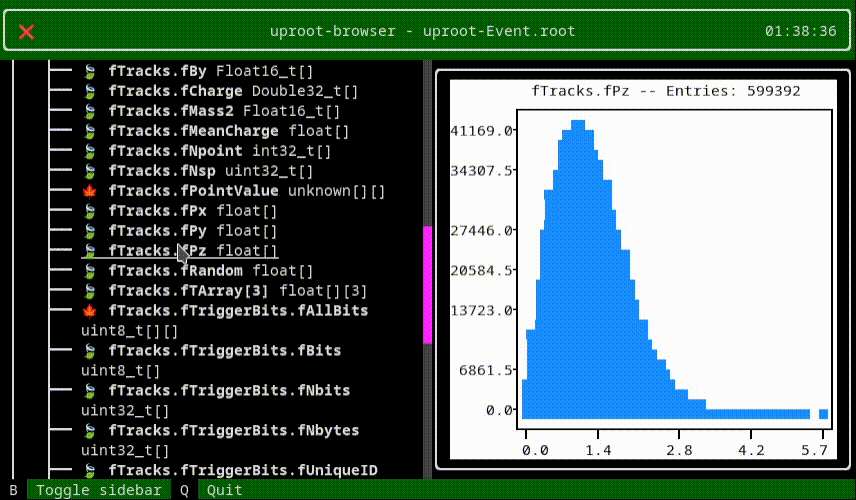
\includegraphics[width=0.9\linewidth]{PLOTS/uproot-browser-tui-frames/15.png}}\only<17>{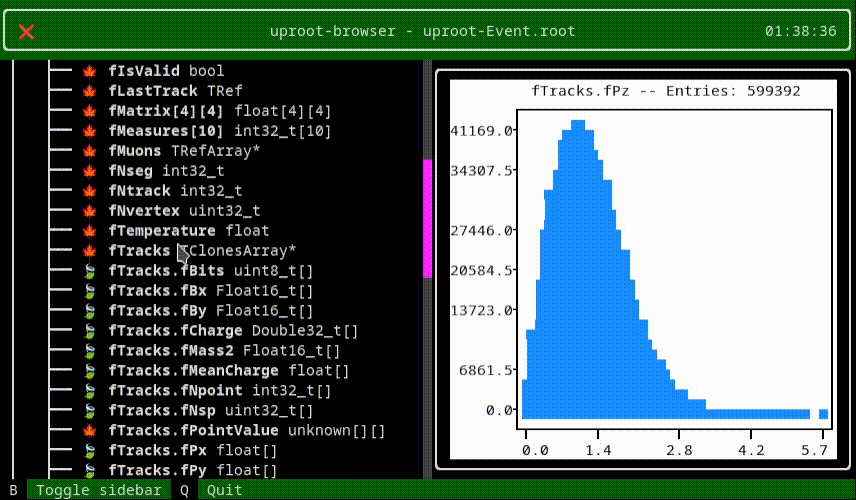
\includegraphics[width=0.9\linewidth]{PLOTS/uproot-browser-tui-frames/16.png}}\only<18>{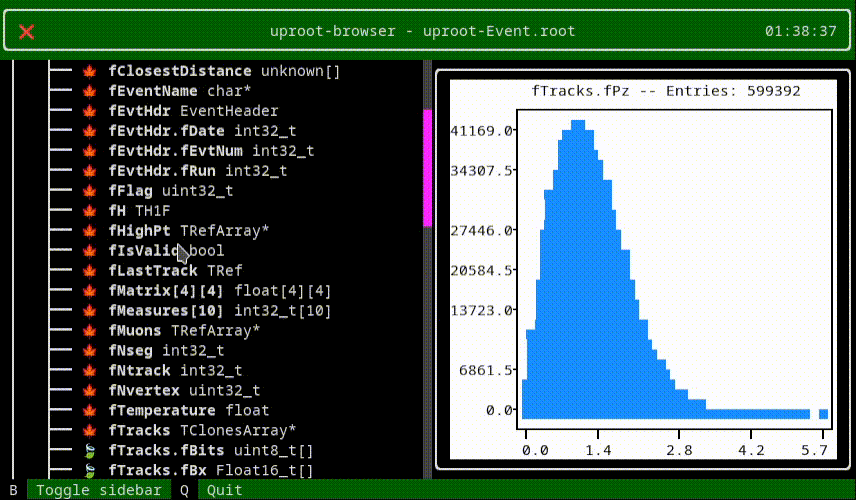
\includegraphics[width=0.9\linewidth]{PLOTS/uproot-browser-tui-frames/17.png}}\only<19>{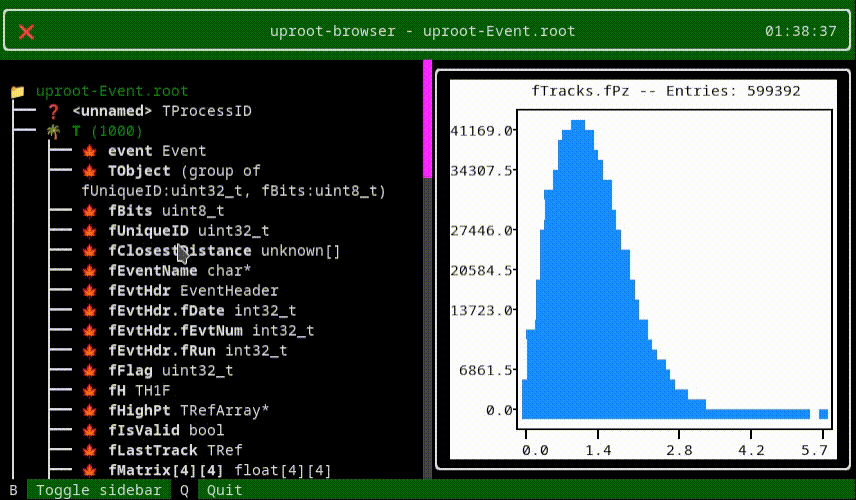
\includegraphics[width=0.9\linewidth]{PLOTS/uproot-browser-tui-frames/18.png}}\only<20>{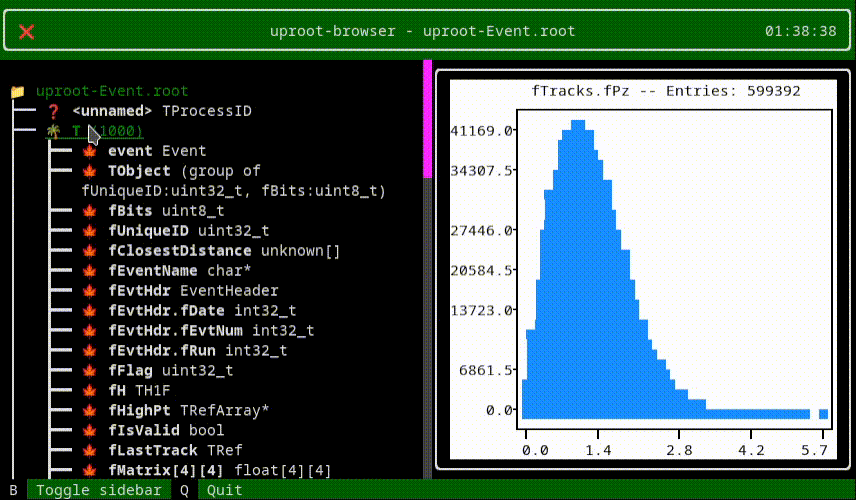
\includegraphics[width=0.9\linewidth]{PLOTS/uproot-browser-tui-frames/19.png}}\only<21>{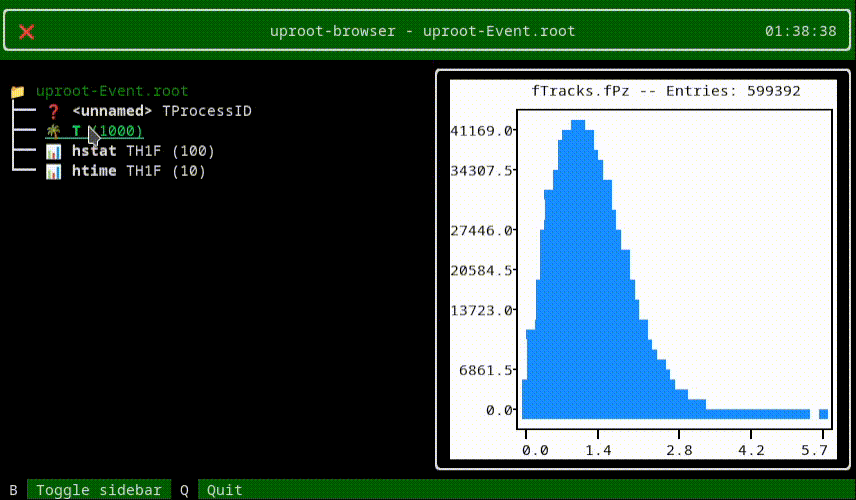
\includegraphics[width=0.9\linewidth]{PLOTS/uproot-browser-tui-frames/20.png}}\only<22>{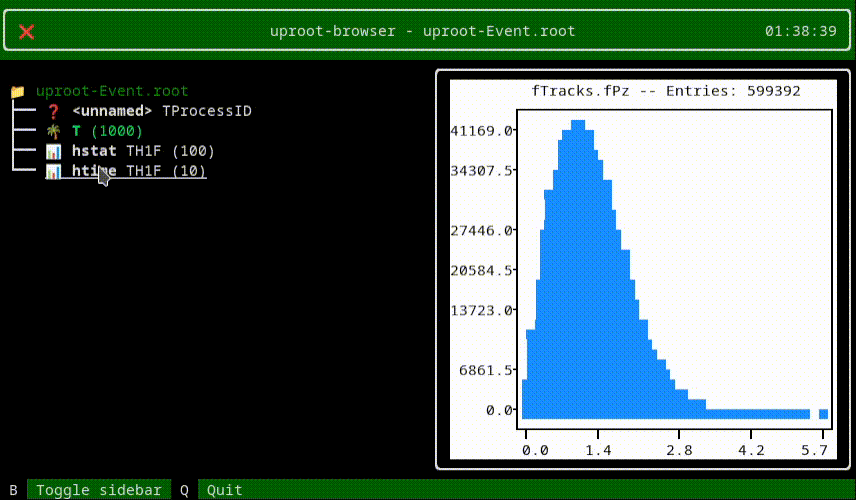
\includegraphics[width=0.9\linewidth]{PLOTS/uproot-browser-tui-frames/21.png}}\only<23>{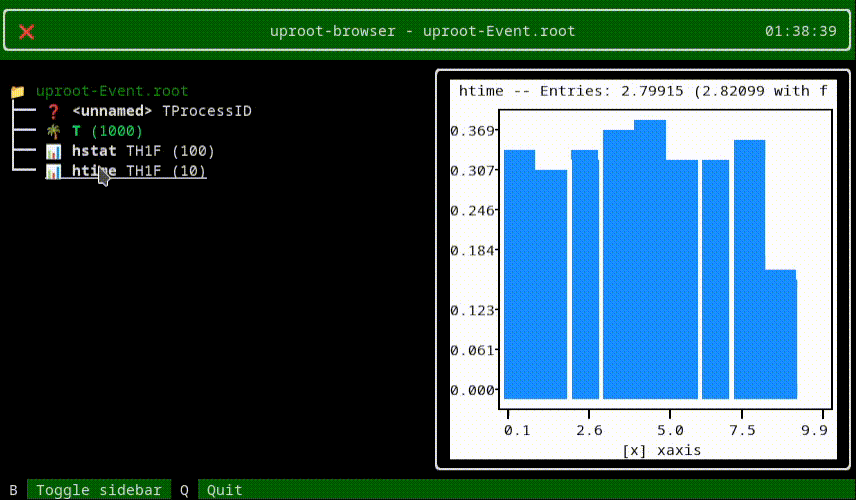
\includegraphics[width=0.9\linewidth]{PLOTS/uproot-browser-tui-frames/22.png}}\only<24>{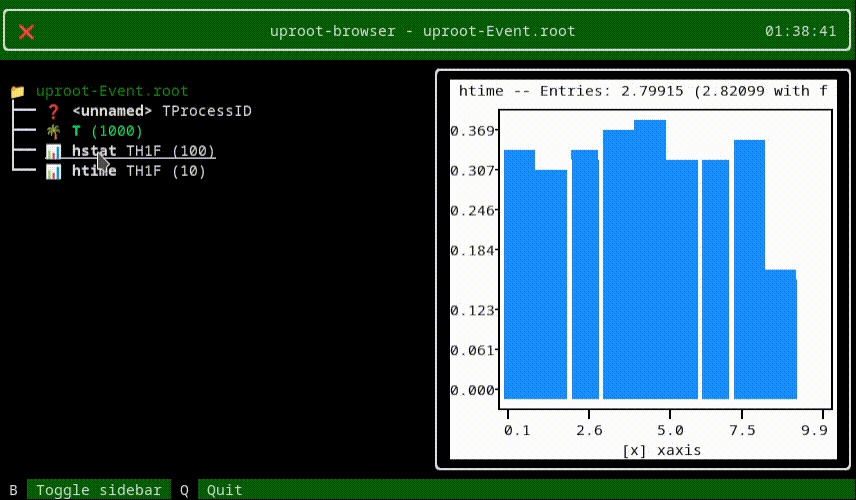
\includegraphics[width=0.9\linewidth]{PLOTS/uproot-browser-tui-frames/23.png}}\only<25>{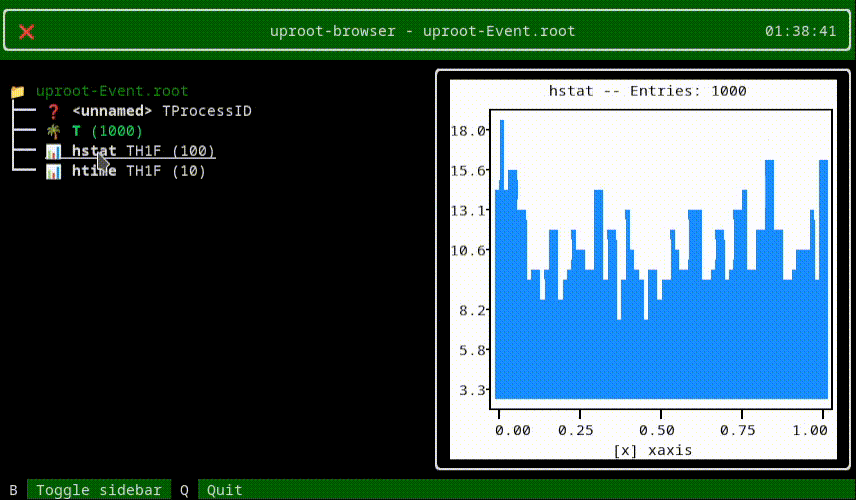
\includegraphics[width=0.9\linewidth]{PLOTS/uproot-browser-tui-frames/24.png}}\only<26>{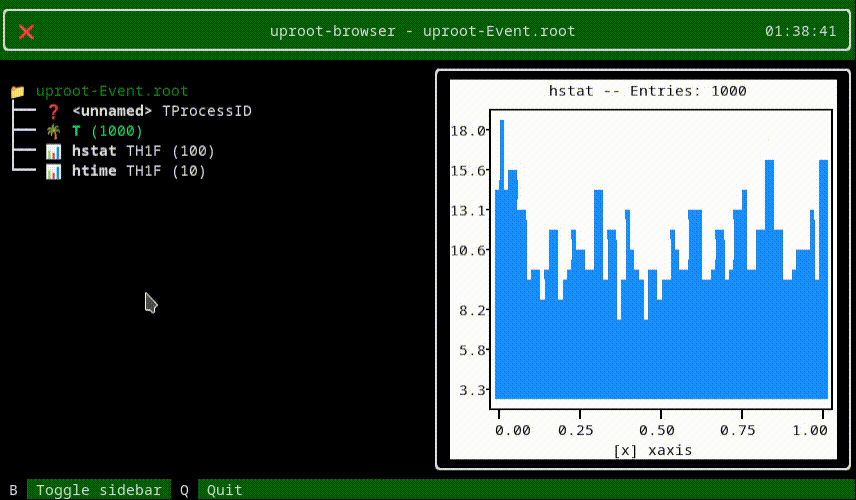
\includegraphics[width=0.9\linewidth]{PLOTS/uproot-browser-tui-frames/25.png}}\only<27>{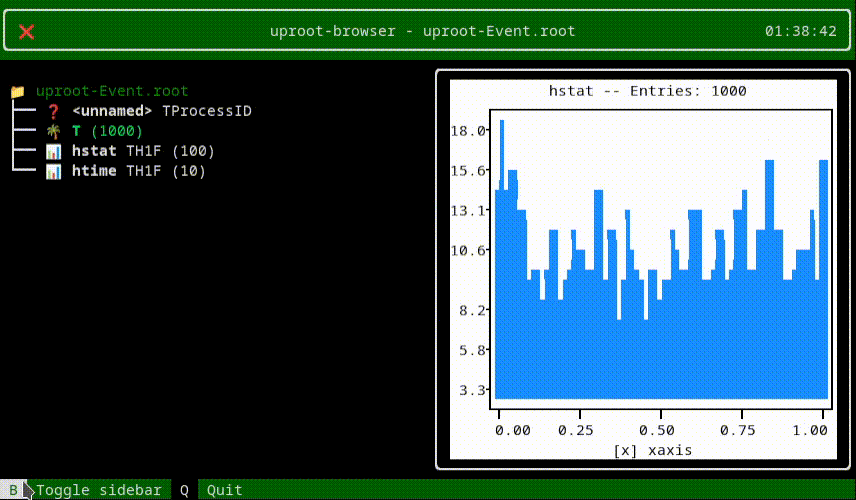
\includegraphics[width=0.9\linewidth]{PLOTS/uproot-browser-tui-frames/26.png}}\only<28>{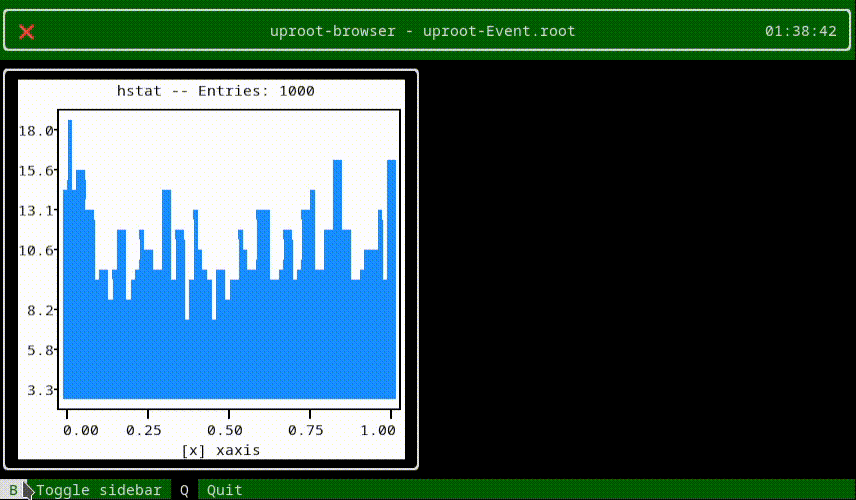
\includegraphics[width=0.9\linewidth]{PLOTS/uproot-browser-tui-frames/27.png}}\only<29>{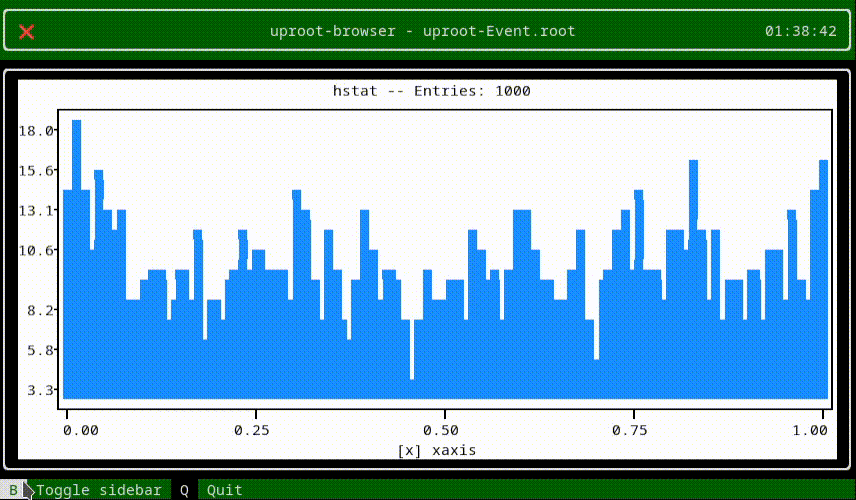
\includegraphics[width=0.9\linewidth]{PLOTS/uproot-browser-tui-frames/28.png}}\only<30>{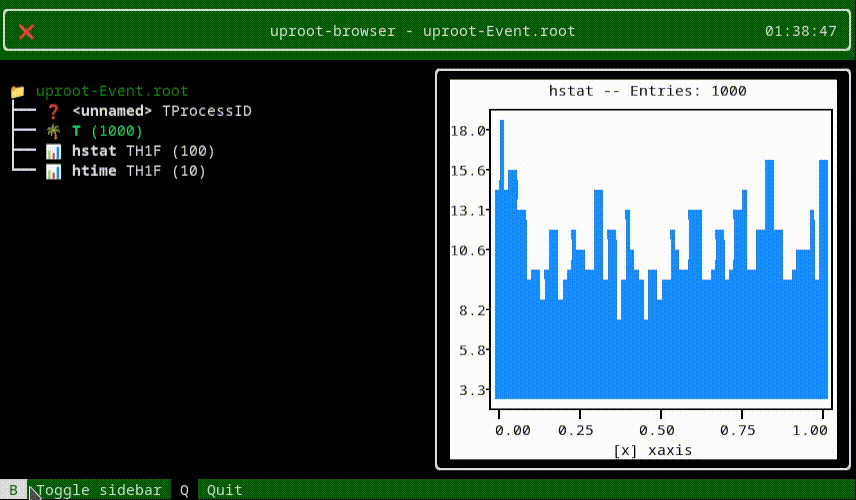
\includegraphics[width=0.9\linewidth]{PLOTS/uproot-browser-tui-frames/29.png}}\only<31>{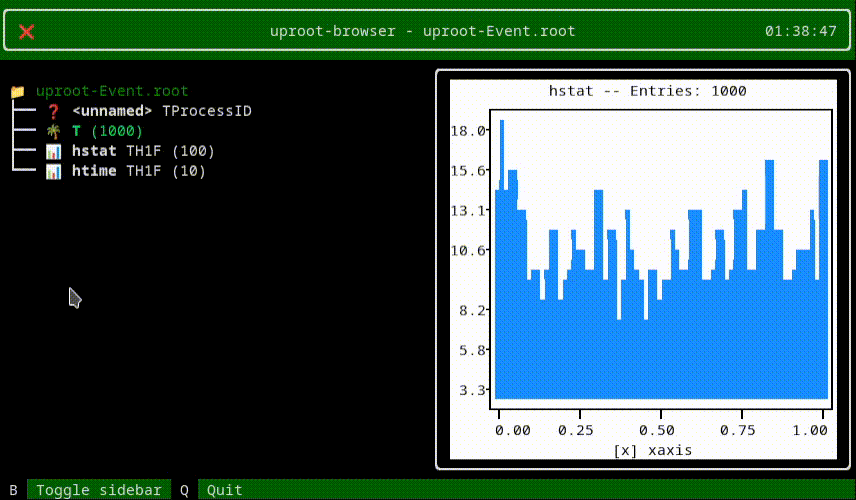
\includegraphics[width=0.9\linewidth]{PLOTS/uproot-browser-tui-frames/30.png}}\only<32>{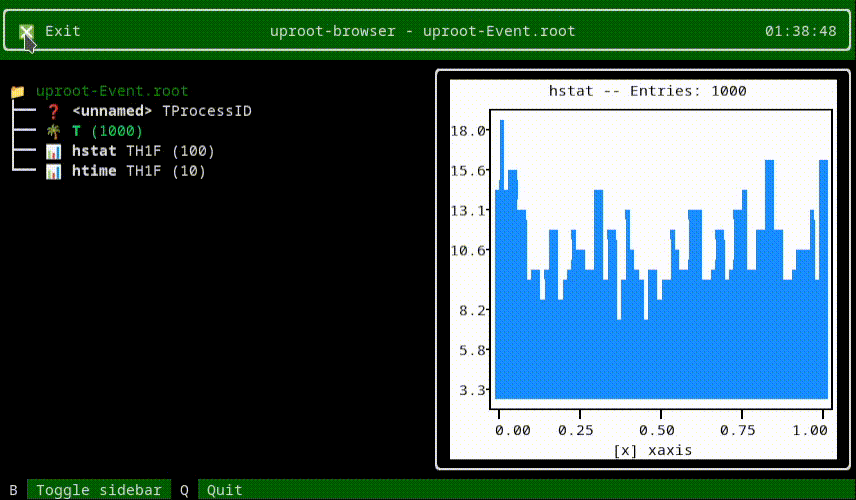
\includegraphics[width=0.9\linewidth]{PLOTS/uproot-browser-tui-frames/31.png}}
\end{center}
\end{frame}

\begin{frame}{Demonstrations of feature-completeness}
\vspace{0.25 cm}
\begin{columns}
\column{0.24\linewidth}
\uncover<2->{My point is not that you {\it should}.}

\vspace{0.75 cm}
\uncover<2->{(Use any tool that gets the job done!)}

\vspace{0.75 cm}
\uncover<2->{My point is that you {\it can}. Scikit-HEP packages cover all aspects of analysis.}

\column{0.75\linewidth}
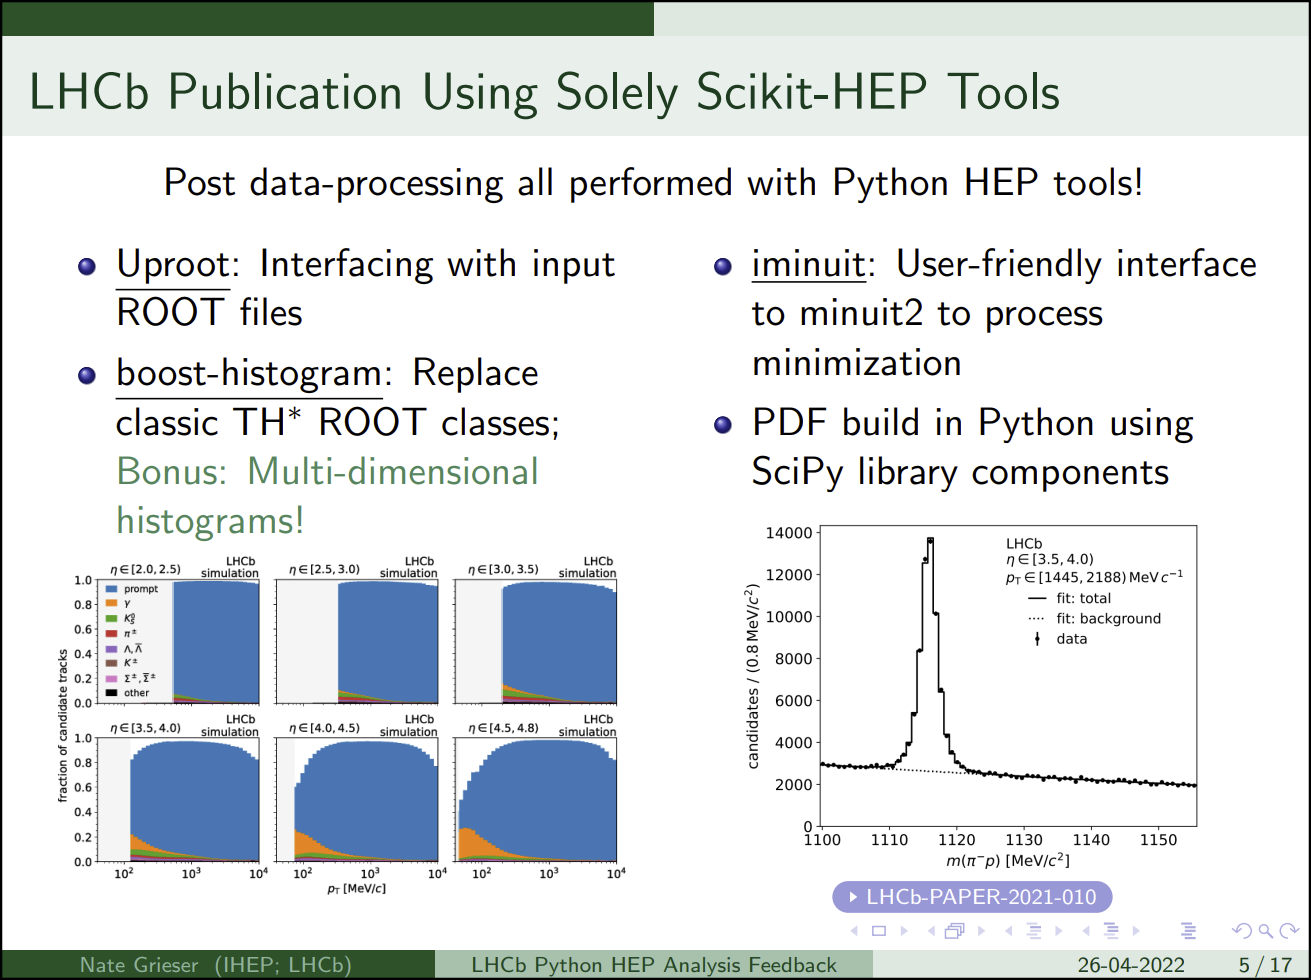
\includegraphics[width=\linewidth]{PLOTS/grieser-lhcb-analysis-in-scikit-hep.png}
\end{columns}
\end{frame}

\begin{frame}{Analysis Grand Challenge (AGC): full-scale test of all components}
\vspace{0.35 cm}
\begin{columns}
\column{1.1\linewidth}
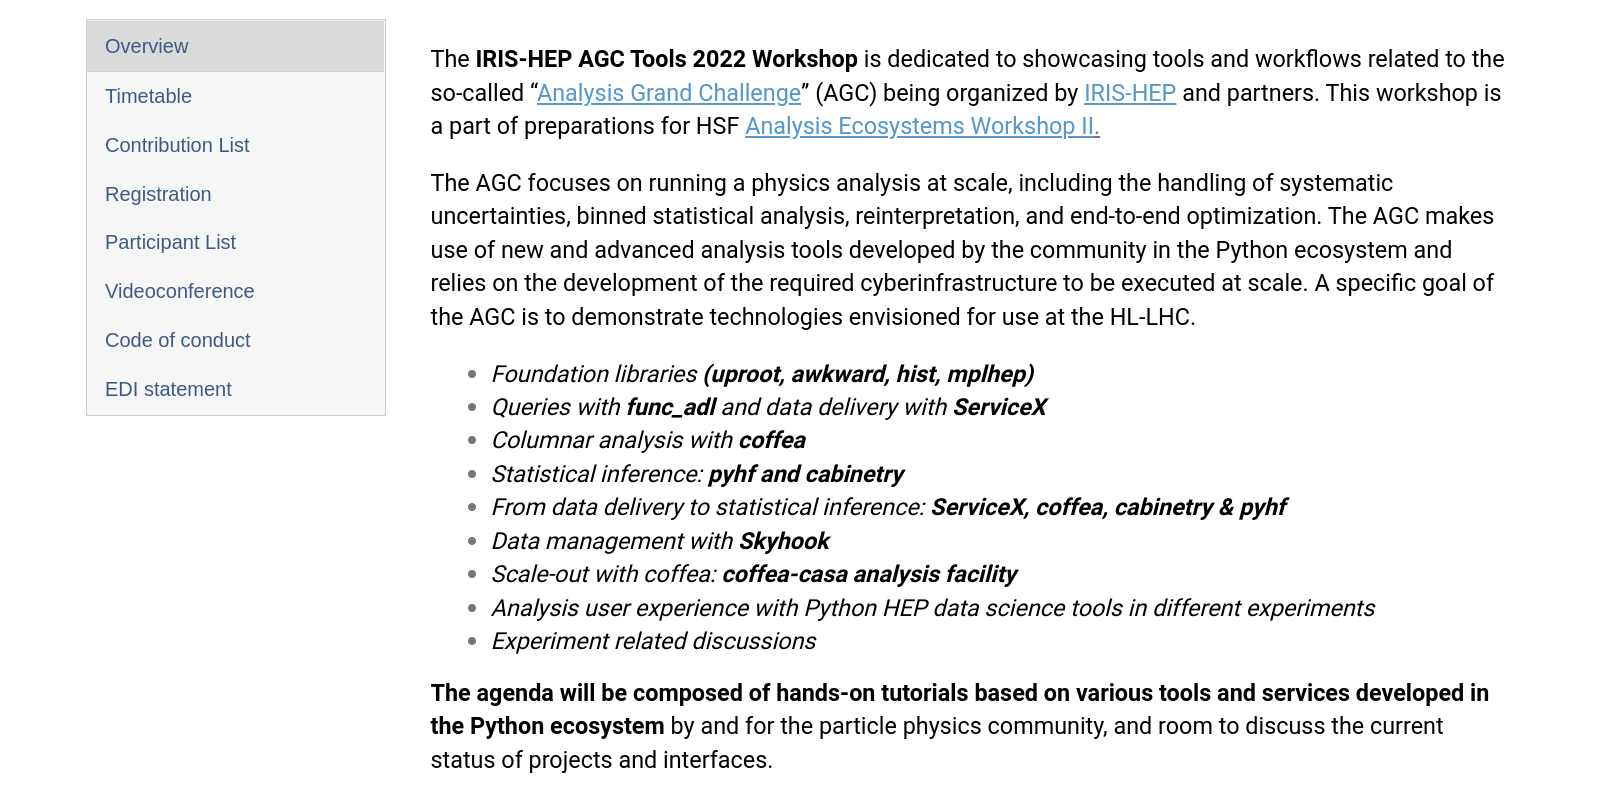
\includegraphics[width=\linewidth]{PLOTS/agc-workshop-2-screenshot.png}
\end{columns}
\end{frame}

\begin{frame}{Analysis Grand Challenge (AGC): full-scale test of all components}
\begin{columns}
\column{0.55\linewidth}
\begin{itemize}\setlength{\itemsep}{0.25 cm}
\item Sample analysis on Run-2 CMS Open Data
\begin{itemize}
\item open data is crucial!
\item currently, MiniAOD $\to$ NanoAOD-like
\item will switch to NanoAOD when available
\item mirrors PHYSLITE
\item thanks to the CMS DPOA team
\end{itemize}

\item Datasets \href{https://github.com/iris-hep/analysis-grand-challenge/tree/main/datasets/cms-open-data-2015}{\textcolor{blue}{listed here}}

\item Everything openly developed
\begin{itemize}
\item \href{https://github.com/iris-hep/analysis-grand-challenge}{\textcolor{blue}{github:iris-hep/analysis-grand-challenge}}
\end{itemize}

\item Using coffea-casa analysis facilities at \href{https://coffea-opendata.casa/}{\textcolor{blue}{UNL}}, \href{https://coffea.af.uchicago.edu/}{\textcolor{blue}{UChicago}}, \href{https://analytics-hub.fnal.gov/}{\textcolor{blue}{Fermilab}}
\end{itemize}

\column{0.528\linewidth}
\fbox{\begin{minipage}{\linewidth}
\begin{description}
\item[Nov 2021:] demo at \href{https://indico.cern.ch/e/agc-tools-workshop}{\textcolor{blue}{first AGC workshop}}
\item[Apr 2022:] second \href{https://indico.cern.ch/e/agc-tools-2}{\textcolor{blue}{second AGC workshop}}
\item[mid 2022:] benchmarking of components
\item[spring 2023:] full scale challenge
\end{description}

\vspace{0.5 cm}
\href{analysis-grand-challenge@iris-hep.org}{\textcolor{blue}{analysis-grand-challenge@iris-hep.org}} (\href{https://groups.google.com/a/iris-hep.org/g/analysis-grand-challenge}{\textcolor{blue}{sign up}})
\end{minipage}}
\end{columns}
\end{frame}

\begin{frame}{Sample $t\bar{t}$ analysis: open data delivery $\to$ inference in a notebook}
\vspace{0.25 cm}
\begin{columns}
\column{0.234\linewidth}
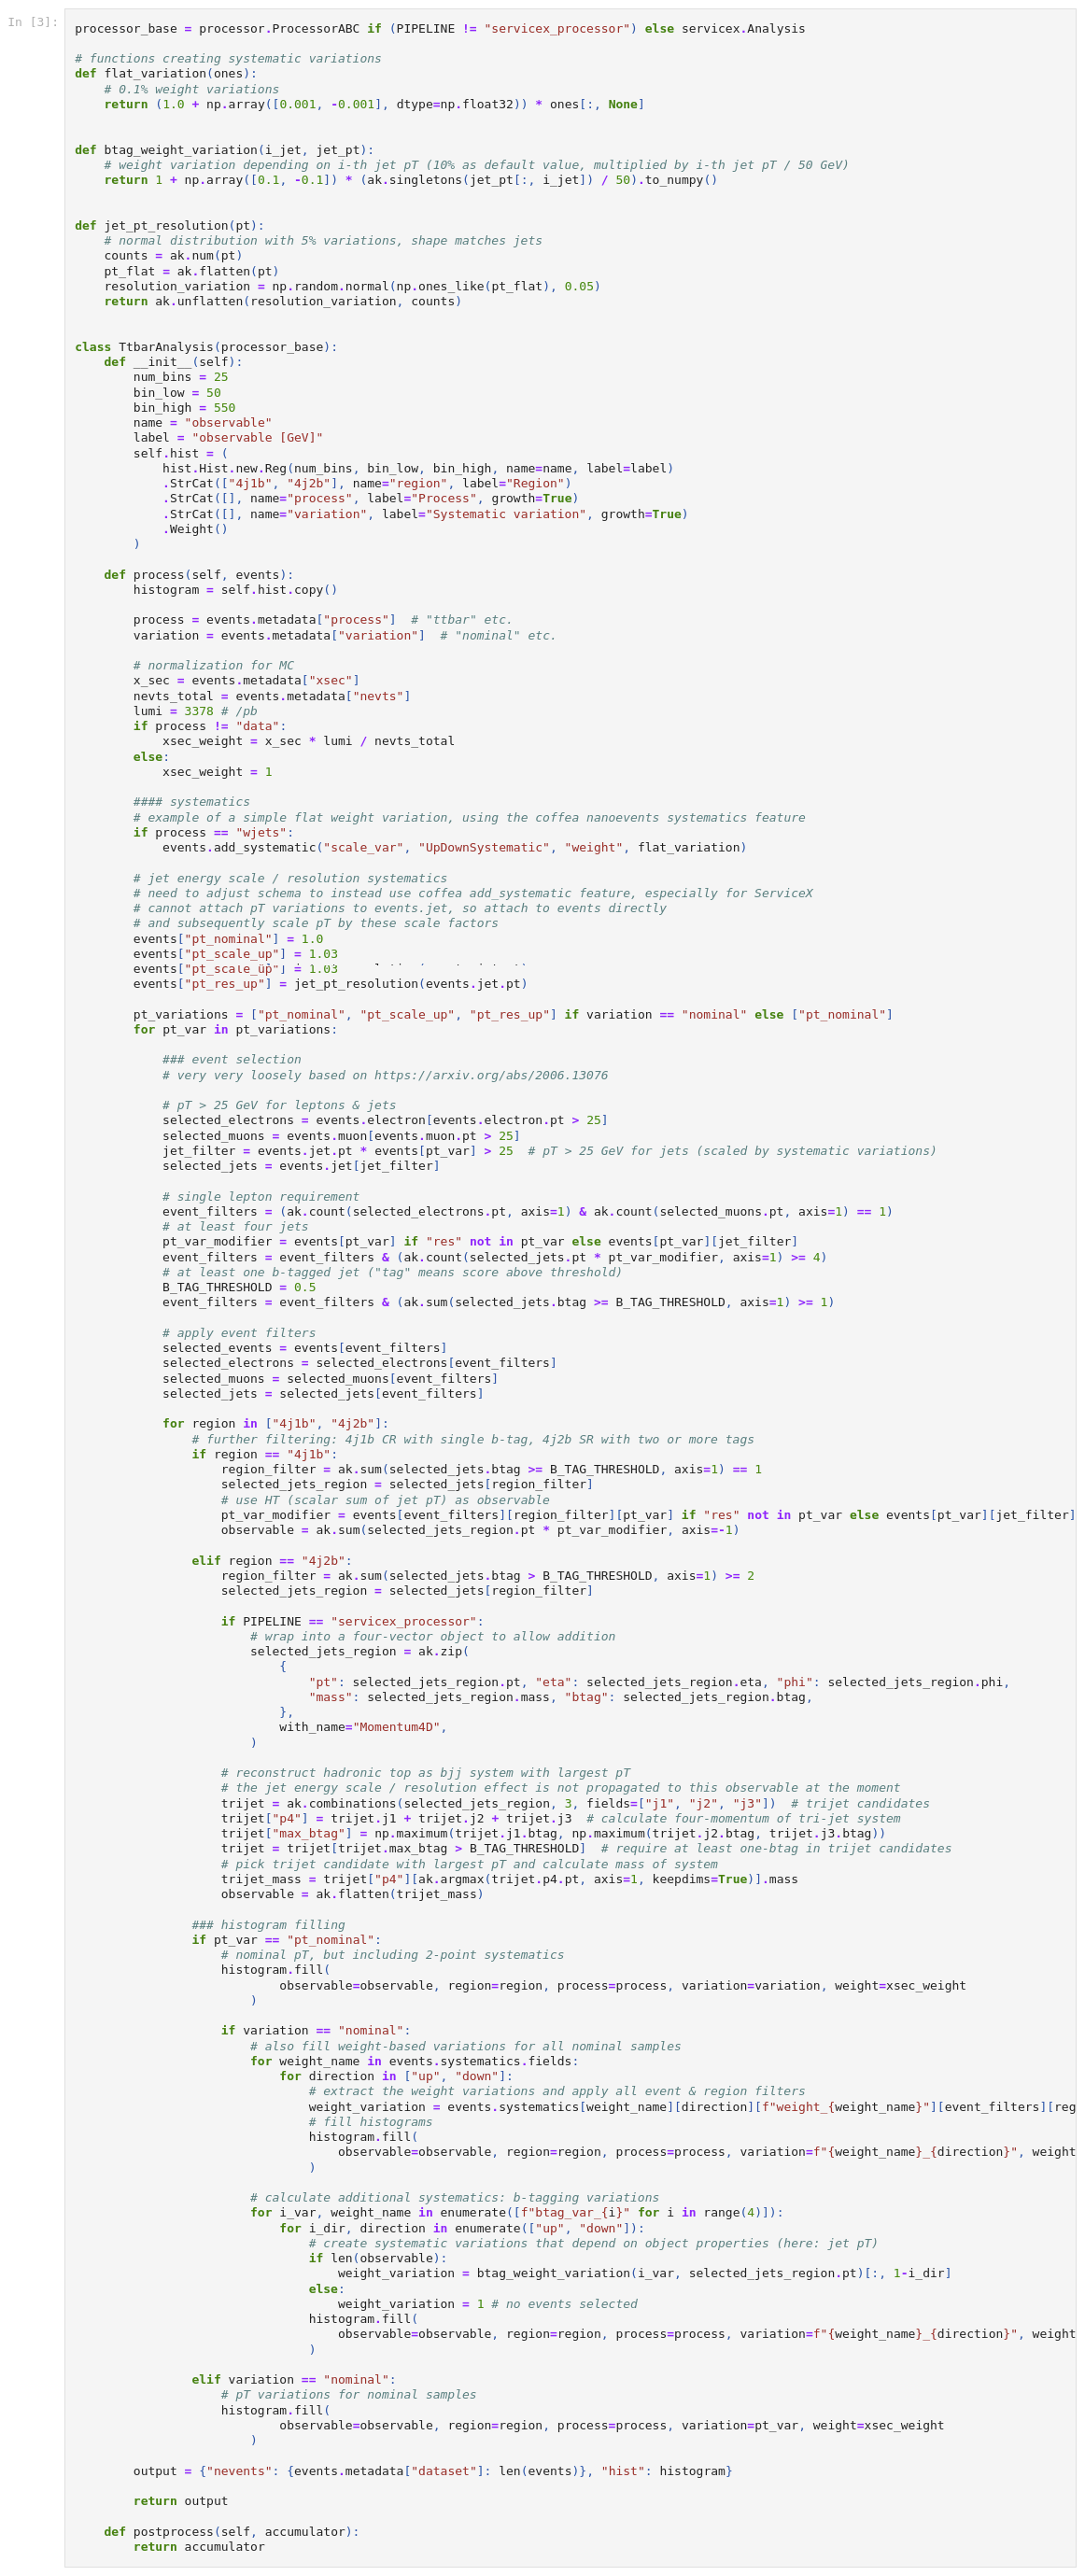
\includegraphics[width=\linewidth]{PLOTS/gac-ttbar-analysis-code.png}

\column{0.01\linewidth}
\column{0.63\linewidth}
\begin{columns}
\column{0.35\linewidth}
\includegraphics[width=\linewidth]{PLOTS/gac-ttbar-plot-0.png}

\vfill
\includegraphics[width=\linewidth]{PLOTS/gac-ttbar-plot-3.png}

\vfill
\includegraphics[width=\linewidth]{PLOTS/gac-ttbar-plot-6.png}

\column{0.37\linewidth}
\includegraphics[width=\linewidth]{PLOTS/gac-ttbar-plot-1.png}

\vfill
\includegraphics[width=\linewidth]{PLOTS/gac-ttbar-plot-4.png}

\vfill
\includegraphics[width=\linewidth]{PLOTS/gac-ttbar-plot-7.png}

\column{0.32\linewidth}
\includegraphics[width=\linewidth]{PLOTS/gac-ttbar-plot-2.png}

\vfill
\includegraphics[width=\linewidth]{PLOTS/gac-ttbar-plot-5.png}

\vfill
\includegraphics[width=\linewidth]{PLOTS/gac-ttbar-plot-8.png}

\end{columns}
\column{0.01\linewidth}
\end{columns}
\end{frame}

\begin{frame}{More AGC tutorials: electroweakinos from funcX to pyhf/cabinetry}
\vspace{0.2 cm}
Laundry list of systematics

\mbox{ } \hfill \includegraphics[width=0.77\linewidth]{PLOTS/agc-electroweakino-pulls.png} \hfill \mbox{ }

Reproduce the published plot (in a {\it tutorial})

\mbox{ } \hfill \includegraphics[width=0.77\linewidth]{PLOTS/agc-electroweakino-likelihood.png} \hfill \mbox{ }
\end{frame}

\begin{frame}{AGC tests connections between services and tools}
\vspace{0.35 cm}
\begin{columns}
\column{1.1\linewidth}
\includegraphics[width=\linewidth]{PLOTS/agc-intersection-of-services-and-tools.png}
\end{columns}
\end{frame}

\begin{frame}{AGC tests connections between services and tools}
\vspace{0.35 cm}
\begin{columns}
\column{1.1\linewidth}
\includegraphics[width=\linewidth]{PLOTS/agc-intersection-of-services-and-tools-2.png}
\end{columns}
\end{frame}

\begin{frame}{Conclusions: what we talked about 5 years ago is happening now}
\vspace{0.25 cm}
\begin{center}
\includegraphics[width=0.77\linewidth]{PLOTS/scikit-hep-in-2017.png}
\end{center}

\vspace{-1.5 cm}
\hfill \mbox{Eduardo Rodrigues\hspace{-0.5 cm}}
\vspace{1.5 cm}
\end{frame}

\begin{frame}{Conclusions: what we talked about 5 years ago is happening now}
\vspace{0.25 cm}
\begin{center}
\includegraphics[width=0.77\linewidth]{PLOTS/gerhard-raven-in-2017.png}
\end{center}

\vspace{-1.25 cm}
\hfill \mbox{Gerhard Raven\hspace{-0.5 cm}}
\vspace{1.25 cm}
\end{frame}

\begin{frame}{Conclusions: what we talked about 5 years ago is happening now}
\vspace{0.25 cm}
\begin{columns}
\column{0.1\linewidth}
\hfill \textcolor{darkblue}{\LARGE 2017}

\column{0.85\linewidth}
\includegraphics[width=\linewidth]{PLOTS/linq-in-2017.png}
\end{columns}

\vspace{0.5 cm}
\begin{columns}
\column{0.1\linewidth}
\hfill \textcolor{darkblue}{\LARGE today}

\column{0.85\linewidth}
\includegraphics[width=\linewidth]{PLOTS/linq-in-2022.png}
\end{columns}

\vspace{0.25 cm}
\hfill \mbox{Gordon Watts\hspace{-0.5 cm}}
\vspace{-0.25 cm}
\end{frame}

\begin{frame}{Conclusions: what we talked about 5 years ago is happening now}
\vspace{0.15 cm}
\begin{center}
\includegraphics[width=0.73\linewidth]{PLOTS/awkward-in-2017.png}
\end{center}

\vspace{-1.25 cm}
\hfill \mbox{embryonic Awkward Array\hspace{-0.5 cm}}
\vspace{1.25 cm}
\end{frame}

\begin{frame}{Conclusions: what we talked about 5 years ago is happening now}
\vspace{0.5 cm}

\includegraphics[width=\linewidth]{PLOTS/af-dream-to-reality.pdf}
\end{frame}

\end{document}
